\documentclass[oneside, openany]{book}
\usepackage[utf8]{inputenc}
\usepackage[backend=bibtex]{biblatex}
\usepackage{amssymb, amsmath, mathtools}
\newtheorem{definition}{Definition}

\usepackage[left=1in, right=1in, top=1in, bottom=1in, includefoot, headheight=13.6pt]{geometry}
\usepackage[T1]{fontenc}

\usepackage{algorithm}
\usepackage[noend]{algpseudocode}
\renewcommand{\algorithmicrequire}{\textbf{Input:}}
\renewcommand{\algorithmicensure}{\textbf{Output:}}

\usepackage{graphicx}
\usepackage{subcaption}
\usepackage{tikz}

\usepackage{url}

\let\cleardoublepage=\clearpage

\addbibresource{TFM.bib}

\begin{document}

\chapter{Introduction}
\label{ch:Introduction}

\section{Deep Learning Models}

\subsection{Multilayer Perceptrons}
A Multilayer Perceptron (MLP), also known as feedforward neural network, is a mathematical model mainly used in supervised learning. Essentially, an MLP is a directed acyclic graph which represents the composition of functions. Each function or \textbf{layer} is a collection of neurons. A neuron is defined as:

\begin{equation}
    \label{eqn:neuron}
    y = f(\mathbf{x}; \theta) = \omega^T \mathbf{x} + b, \qquad \theta = (\omega, b)
\end{equation}

The term \textit{perceptron} refers to a linear classifier consisting of one layer \cite{rosenblatt1958}, $f(\mathbf{x}; \theta) = \mathbb{I}(\omega^T \mathbf{x} + b > 0)$.
Here, $\mathbb{I}(a>0)$ is the Heaviside function, which is non-differentiable. In MLP, the activation function from the original perceptron $\mathbb{I}$ is usually replaced by another differentiable function $\psi \colon \mathbb{R} \to \mathbb{R}$. The internal layers of MLP are usually named \textbf{hidden layers}, the last one is called \textbf{output layer}. The dimensionality of the hidden layers determines the \textbf{width} of the neural network \cite{goodfellow2016}. Each layer $l$ consists of many units $\mathbf{z}_l$ which are computed as a linear transformation of the units from the previous layer $l-1$ passed element-wise through the activation function \cite{murphy2022}:
\begin{equation*}
    \mathbf{z}_l = \psi_l (\mathbf{W}_l \mathbf{z}_{l-1} + \mathbf{b}_l)
\end{equation*}

We can choose different activation functions that will define our model and impact in the performance of the training. If we use a linear activation function $\psi_l (x) = K_l x$ then our neural network becomes just a linear model \cite{murphy2022}, that's why usually non-linear activation functions are used, since we would like to capture non-linear relationships between the input data and the output. Also, the Universal Approximation Theorem states that a neural network with a single hidden layer and non-linear activation functions can approximate any continuous function on a compact subset of $\mathbb{R}^n$ to any desired degree of accuracy.
Since the goal of an MLP is to approximate some function $f^*$ (for example, for a classifier $y = f^*(\mathbf{x})$), non-linear activation functions are necessary to achieve this level of approximation.
However, they can be used when we know the problem is linearly separable (think of two separate clusters of points in $\mathbb{R}^2$ in a classifier model) or in the output layer, for example when the MLP acts as a regression model.\\
If we change the Heaviside function by the sigmoid (logistic) function $\sigma(x) = \frac{1}{1+e^{-x}}$ we get a smooth approximation of $\mathbb{I}$. Another choice of activation function could be $tanh(x) = \frac{e^x - e^{-x}}{e^x + e^{-x}}$ which has a similar shape but its image is $(-1,1)$. Both are valid activation function and have been used. However, since we need to compute gradients in the optimization process in order to update the weights, a $\mathbf{0}$ gradient would be a problem, since it will make hard to train a model using gradient descent (vanishing gradient problem).
Both functions have an almost horizontal slope (gradient near 0) for large positive and negative inputs. Also, $\lVert \frac{d}{dx} \sigma(x) \rVert = \lVert \sigma(x)(1-\sigma(x)) \rVert \leq \frac{1}{4} < 1$, therefore several multiplications will quickly approximate to zero. Although they are used in practice (for example, $\sigma(\cdot)$ is used in the output layer for binary regression problems), in order to train deep models we need non-saturating activation functions for the hidden layers.
One of the most used is \textit{rectified linear unit}: $ReLU(x) = \max (a,0) = a \mathbb{I}(a>0)$. The gradient of $ReLU'(z) \neq 0$ as long as $z$ is positive: this function don't require input normalization to prevent them from saturating.
As stated in \cite*{glorot2011}, the rectifier activation function allows a network to easily obtain sparse representations, the \textit{hard} saturation (gradients being exactly 0) help supervised training: experimental results suggest that networks with ReLU activation functions in the hidden layers have better convergence performance than using sigmoid \cite{krizhevsky2017}.
There has been a lot of activation functions proposed in the last years, [TERMINAR ESTO] .\\

The neural network tries to approximate the target function $\mathbf{y} = F(\mathbf{x})$, the \textit{true} relation between the variables. The network, $f(x;\theta)$, \textit{learns} by searching the parameters $\boldsymbol{\theta}$ that minimizes a loss function $J(\boldsymbol{\theta})$, which measures the distance between the output and the target or the proximity between probability densities of random variables \cite*{calin2020}. If we consider a $k$-class classification problem with $\mathcal{X} \subset \mathbb{R}^d$ the feature space and $\mathcal{Y} = \{1,\dots, k\}$ the label space, given the dataset $D = \{(\mathbf{x}_1, y_1),\cdots,(\mathbf{x}_n, y_n)\}$ and a MLP $f\colon \mathcal{X} \to \mathbb{R}^k$ with a softmax as the output layer.
For any loss function $J(\boldsymbol{\theta}) = J(f(\mathbf{x}, \boldsymbol{\theta}), y)$, assuming there is a joint distribution $P(\mathbf{x},y)$ over $\mathcal{X}$ and $\mathcal{Y}$, the \textbf{risk} of $f$ is defined as $R_J (f) = \mathbb{E}\Bigl[ J(f(\mathbf{x}; \boldsymbol{\theta}), y) \Bigr] = \int J(f(\mathbf{x}; \theta), y) dP(\mathbf{x}, y)$ and the \textbf{empirical risk} is defined as $\hat{R}_J (f) = \mathbb{E}_D \Bigl[ J(f(\mathbf{x}; \boldsymbol{\theta}), y) \Bigr]$ assuming that $\{(\mathbf{x}_i, y_i)\}_{i=1}^n$ are IID samples from $P(\mathbf{x}, y)$.
Since the nonlinearity of an MLP makes the loss function to become non-convex, it's trained using iterative, gradient-based optimizers. Most neural networks, and in particular the models that will be used in this work, are trained using maximum likelihood: the loss function is the negative log-likelihood \footnote{Empirical risk minimization is equivalent to Maximum Likelihood Estimation when the risk is defined as the negative of the likelihood. Note that ERM does not limit itself to that particular class of risk functions.} \cite{goodfellow2016}. That is, we will compute the \textit{cross-entropy}\footnote{This is valid for a loss consisting of a negative log-likelihood, not only for the negative log-likelihodd of a softmax distribution.} between the training data and the model distribution:

\begin{equation}
    J(\theta) = -\mathbb{E}_{\mathbf{x}, y \sim D} \log_{P(\mathbf{x}, y)} (y | \mathbf{x})
\end{equation}
In a $k$-class classification model with a cross-entropy loss function, the empirical risk to minimize is $\hat{R}_J (f) = -\frac{1}{n}\sum_{i=1}^n \sum_{j=1}^k \mathbf{y}_{ij} \log f_j (\mathbf{x}_i; \boldsymbol{\theta})$, where $\mathbf{y}_{ij}$ is the j-th element of the one-hot encoded label of $\mathbf{x}_i$ such that $\mathbf{1}^T \mathbf{y}_i = 1$, $\forall i$, and $f_j$ is the j-th element of the softmax output layer of $f$ \cite{zhang2018}.\\
Typically, the minimization of $J(\boldsymbol{\theta})$ is achieved using a gradient descent algorithm. Large training datasets are good for generalization, but since $\nabla_{\boldsymbol{\theta}} J (\boldsymbol{\theta}) \frac{1}{n}\sum_{i=1}^n \nabla_{\boldsymbol{\theta}} l(f(\mathbf{x}; \boldsymbol{\theta}), y)$ has a computational complexity of $\mathcal{O}(n)$ for each step \cite{goodfellow2016}, this approach is prohibitive for $n$ in a scale of millions. Optimization algorithms that use the whole dataset are called \textbf{batch}\footnote{The term \textit{batch} may also refer to a subset of the training set. The size of a minibatch is usually called \textit{batch size}.} gradient methods.
When only a single sample is used each step, the method is called \textbf{stochastic}. The \textbf{Minibatch Stochastic Gradient Descent} (MSGD) algorithm (and its variants) is preferred, since the gradient direction in SGD oscillates because of the additional noise added by random sampling \cite{sun2019}.
The MSGD algorithm makes and estimation of the gradient selecting randomly a \textit{minibatch} $b = \{(\mathbf{x}, y)^{(1)},\cdots, (\mathbf{x}, y)^{(m)}\}$, $m<n$ such as:

\begin{equation}
    \label{eqn:gradient_estimate}
    \mathbf{g} = \frac{1}{m} \nabla_{\boldsymbol{\theta}} \sum_{i=1}^m l(f(\mathbf{x}^{(i)}; \boldsymbol{\theta}), y^{(i)})
\end{equation}

Each step of the MSGD algorithm, the parameters $\boldsymbol{\theta}$ are updated given a learning rate $\eta > 0$: $\boldsymbol{\theta} = \boldsymbol{\theta} - \eta \mathbf{g}$. A constant learning rate during training may lead to a zone where the gradient estimate "jumps around" a local minimum, although if the network is complex enough to represent the underlying function, a constant learning rate usually works well in practice \cite{sun2019a}. In some implementations, the learning rate is updated during training, an example could be multiplying by a factor $0<\gamma<1$ each $T$ number of steps\footnote{This is actually what the \textit{StepLR} class does in the popular Python package torch.optim.}.
Here, we encounter some challenges \cite{ruder2017}:

\begin{itemize}
    \item A small $\eta$ leads to slow convergence of vanilla MSGD, while if it's too large the loss function will fluctuate around the minimum or diverge.\\
    \item A learning rate scheduler needs to be defined at the beginning and it's not adapted to dataset's characteristics.\\
    \item Since $J(\boldsymbol{\theta})$ is non-convex (recall that affine transformations followed by an activation function such as ReLU is non-covex). A key challenge is avoiding getting trapped in suboptimal local minima. Also, according to \cite{dauphin2014}, the difficulty comes from saddle points present in high-dimensional non-convex optimization that are hard for SGD to scape, since the gradient is close to zero in all dimensions.
\end{itemize}

There are several gradient-based variants that try to tackle these challenges. For example, a momentum term can be used to help accelerate MSGD and dampen oscillations \cite{qian1999}.
Momentum stores the gradient of the past step to adjust the new direction:

\begin{align}
    \label{eqn:SGD_momentum}
    \begin{split}
    \mathbf{v}_t &= \alpha \mathbf{v}_{t-1} + \eta \nabla_{\boldsymbol{\theta}} J(\boldsymbol{\theta}) \qquad \eta>0, \hspace*{.3 em} \alpha \in [0,1] \\
    \boldsymbol{\theta} &= \boldsymbol{\theta} - \mathbf{v}_t
    \end{split}
\end{align}

The momentum term increases the updates for dimensions whose gradients point in the same direction, allowing the algorithm to build momentum and move more efficiently towards the minimum. Conversely, it reduces updates for dimensions whose gradients change direction, dampening out oscillations and preventing the algorithm from getting stuck in local minima \cite{ruder2017}.\\

Another variant is \textbf{Nesterov accelerated gradient} \cite{y1983}, which is an extension of Gradient Descent with momentum where the computation of the gradient is performed using projected parameters and not the actual values:

\begin{align}
    \label{eqn:Nesterov_accelerated_gradient}
    \begin{split}
        \mathbf{v}_t &= \alpha \mathbf{v}_{t-1} + \eta \nabla_{\boldsymbol{\theta}} J(\boldsymbol{\theta} - \alpha \mathbf{v}_{t-1}) \\
        \boldsymbol{\theta} &= \boldsymbol{\theta} - \mathbf{v}_t
    \end{split}
\end{align}

Here, similar to GD with momentum, $\mathbf{v}_t$ is the direction and speed at which the parameters should be tweaked and $\alpha$ determines how quickly the previous gradients will decay. Nesterov Accelerated Gradient tries to tackle the exploding gradient case: where the velocity added to the parameters gives an unwanted high loss. In this case, if the velocity update lead to a bad loss, the gradients will redirect the update back to $\boldsymbol{\theta}$.

[PONER IMAGEN QUE COMPARE MOMENTUM CON NAG]

Still, with the previous algorithms the hyperparameters $\eta$ and $\alpha$ need to be fixed or changed during training a heuristic way. With the \textbf{Adaptative Gradient Algorithm} (\textbf{Adagrad}), the learning rate change depending on the parameters: it performs larger updates for infrequent parameters and smaller updates for frequent parameters. That's it, each parameter is updated with a different learning rate each step.
We set $g_{t,i}$ the gradient estimate w.r.t the parameter $\theta_i$ at step $t$. The Adagrad update rule is:

\begin{equation}
    \theta_{t+1, i} = \theta_{t,i} - \frac{\eta}{\sqrt{G_{t,i} + \epsilon}} g_{t,i}
\end{equation}

Where $G_{t,i}$ is the sum of squares of the gradients w.r.t $\theta_i$ up to step $t$, and $\epsilon > 0$ is the decimal smallest number in the machine, in order to avoid division by zero. With Adagrad, the selection of $\eta$ is irrelevant since the term will be scaled by the root. Most implementations just fix it at $0.01$. The problem with this algorithm is that the accumulated sums will increase during training and eventually the learning rate will be close to zero, therefore the parameters are not updated at a certain point.
In order to fix this, \textbf{Adadelta} restricts the number of accumulated gradients to some fixed size.

\subsection{Convolutional Neural Networks}


\section{Other ML models}

\chapter{Federated Learning}
\label{ch:Federated_Learning}

\section{Introduction}
In the rapidly evolving landscape of artificial intelligence and machine learning, Federated Learning (FL)
has emerged as a paradigm that addresses key challenges related to privacy, data security,
 and decentralized computing. Federated Learning represents a novel approach to model training, allowing
 machine learning models to be trained collaboratively across multiple decentralized devices or servers
 without exchanging raw data \cite{mcmahan2023a}.

 Unlike traditional centralized approaches, where data is collected and processed in a central server, FL enables training on local devices following a scheme of decentralized model training.
 This decentralization ensures that data remains on the device, granting a certain degree of privacy.
 In a centralized setting, the trained model is updated based on the complete dataset, which is stored in a unique server. In the federated setting, data is distributed across local devices (parties) and training happens locally. This can be problematic, since the source
 of the data differ, the data can differ in various ways: unbalanced datasets, different distributions, etc. This is one of the main challenges of FL:
 \textbf{non-IID data}, since this will negatively affect the performance of the model \cite{li2020}, \cite{zhao2018}, \cite{li2021}.

Horizontal Federated Learning (HFL) and Vertical Federated learning (VFL) are two variations of the federated learning paradigm that differ in how they distribute and collaborate on data.

\begin{itemize}
    \item \textbf{HFL:} Each party has a portion of the overall dataset, each party holds a different subset of samples but for the same features.
    \item \textbf{VFL:} The data  is vertically partitioned, each party has different features for the same set of samples.
\end{itemize}

[\textbf{PONER TABLAS QUE ILUSTREN HFL Y VFL}]

HFL and VFL are not mutually exclusive, in some cases a combination of both schemes may be applied. This work will focus on HFL. Also, we will only study \textit{Cross-Silo Federated Learning (Cross-Silo FL)},
which is a variation of FL that addresses the scenario where data is distributed across different organizations, usually few parties, each maintaining control over its own data.
This setting is particularly relevant in industries where different organizations need to collaborate on machine learning task, such as healthcare (hospitals collaborating on medical research), finance (banks collaborating on fraud detection), epidemiological studies (international public health agencies studying disease spread),
smart cities (urban planning authorities collaborating on public services optimization), etc. Ensuring interoperability between different silos is a huge challenge, since there needs to be a fixed standard in data format, structures and processing capabilities accross different organizations.\\
Another flavour of FL is \textit{Cross device FL}, which was the original topology proposed \cite*{mcmahan2023a}. In this type of setting, the scale of the parties is potentially much bigger (order of millions) since it's aimed to mobile devices, IoT, apps... where the data format and architecture is usually already defined by an organization. For example, this is the kind of FL that Google uses for training Gboard's models \cite*{zhang2023}. With \textit{Cross device FL}, it's needed to take into account some technical difficulties like client selection strategy \cite*{smestad2023}, connection overheard, connection dropouts, device heterogeneity, etc.
Some of these challenges are shared with \textit{Cross-Silo FL}. The main differences are the scale of parties, the computing resources (mobile devices vs data centers or computers) and the partition of data: \textit{cross device} tends to be HFL while \textit{cross-silo} could be HFL or VFL. Since we are focusing in \textit{cross-silo FL}, it won't be studied the implications of client selection (since we are assuming the parties are few and well-defined), the connection overheard or dropouts. The focus of this work will be mainly the statistical heterogeneity challenge, since this work serves as the final project for obtaining a MSc in Statistics.

We will begin by studying the FedAvg algorithm \cite{mcmahan2023a}, which is de facto approach for Federated Learning (FL). We will establish notation, examine some of its properties, and explore issues that arise when data is not independently identically distributed (statistical heterogeneity). Following that, various approaches that have been proposed to address this problem will be developed, and the performance of each will be analyzed across different training architectures.

\section{FedAvg}

Let $D = \{(\mathbf{x}, y)\}$ be the global dataset\footnote{Here, the global dataset is the union of the different local datasets, $D = \cup_{i=1}^N D^i$ . In practical cases, there is no such dataset in order to ensure data privacy. However, we will consider it to conduct a performance study of the various algorithms.} and $D^i \subset D$ the $i$-th party's local dataset, $i=1,...,N$.
Let $\omega_g^t$ and $\omega_i^t$ be the global model and the local model of the $i$-th party in round $t\in \{1,...,T\}$, respectively. Since we are working in a \textit{Cross-silo FL} setting, the main differences between a federated optimization scheme and a distributed one would be the unbalanced data and non-IID data.\\
In a general FL optimization framework, we want to minimize the objective function:

\begin{equation}
\label{eqn:objective}
F(\omega) = \mathbb{E}_{i \sim D}\Big[ F_i (\omega_g) \Big], \qquad F_i(\omega_g) = \mathbb{E}_{z \sim D^i}\Bigl[ l_i (\omega_g, z) \Bigr]
\end{equation}

Here, $l_i(\omega_g, z)$ represents the local loss function of client i (with local dataset $D^i$). As stated in \cite*{wang2021}, the objective function in \ref{eqn:objective}
can take the form of an empirical risk minimization objective function:

\begin{equation}
  \label{eqn:empirical_objective}
  F(\omega_g) = \sum_{i=1}^N \alpha_i F_i(\omega_g) \text{ where } F_i (\omega_g) = \frac{1}{|D^i|} \sum_{z \in D^i} l_i(\omega_g, z) \text{ and } \sum_{i=1}^N \alpha_i = 1
\end{equation}

If $\alpha_i = \frac{|D^i|}{\sum_{i=1}^N |D^i|}$, the objective function in \ref{eqn:empirical_objective} would be the empirical risk minimization objective function of $D = \cup_i D^i$. We recall that \ref{eqn:objective} is an optimization problem that could be solved using Stochastic Descent: $\omega_g^{t+1} = \omega_g^t - \eta_t \nabla F (\omega_g^t)$ where $\eta_t$ is the learning rate at time $t$. In practice, we will use an unbiased estimator of the gradient of the local loss $g_i (\omega_g^t)$ such that $\mathbb{E}_{z \sim D^i} \Bigl[ g_i (\omega_g^t) \Bigr] = \nabla F_i (\omega_g^t)$ using Stochastic Gradient Descent (SGD).

In \cite*{mcmahan2023a}, it was introduced the \textbf{FederatedAveraging} algorithm (FedAvg).

\begin{algorithm}[H]
  \label{alg:FedAvg}
  \caption{FedAvg}
  \begin{algorithmic}[1]
    \Require{local datasets $D^i$ $\forall i \in \{1,\dots, N\}$, number of parties $N$, number of communication rounds $T$, number of local epochs $E$, learning rate $\eta$ for SGD, local mini-batch size $B$.}
    \Ensure{global model $\omega^T_g$.}
    \Statex
    \Procedure{Server execution}{}
    \State Initialize $\omega_g^0$
    \For {round $t = 1,\dots, T$}
      \State $S_t$  (Selection of clients)
      \For {client $k \in S_t$ \textbf{in parallel}}
        \State $\omega_k^{t+1} \gets ClientUpdate(k, \omega_g^t)$
      \EndFor
      \State $\omega_g^{t+1} \gets \sum_{k \in S_t} \frac{|D^k|}{\sum_{k \in S_t} |D^k|} \omega_k^{t+1}$
    \EndFor
    \EndProcedure

    \Procedure{$ClientUpdate(k, \omega_g^t)$}{}
    \State $\omega_k^t \gets \omega_g^t$
    \State $\mathcal{B} \gets$ Batches of $D^k$ of size $B$
    \For {local epoch $i=1,\dots,E$}
      \For {batch $\mathbf{b} \in \mathcal{B}$}
        \State $\omega_k^t \gets \omega_k^t - \eta \nabla l(\omega_k^t; \mathbf{b})$
      \EndFor
    \EndFor
    \State return $\omega_k^t$ to the server.
    \EndProcedure
  \end{algorithmic}
\end{algorithm}

As we see, \textit{FedAvg} took into account a client selection strategy. Since we are focusing in a framework where the clients are limited, we will not consider any subset of clients each round: all the clients will participate.\\
The algorithm is quite simple, the server is simply averaging the local models' weights, with a constant parameter determining the contribution of each client given the size of the local dataset.\\
Each client performs multiple local epochs, which reduces the communication rounds. However, these local updates can lead to a worse performance since the local objective functions differ from each other. This makes the algorithm not robust against non-IID data. There are several works that try to tackle this problem and a lot of FedAvg variants have been proposed in order to mitigate the divergence between the local updates. We will review some of the more relevant of them, starting with \textit{FedProx}.

\section{FedProx}

In \cite*{li2020}, a generalization of \textit{FedAvg} was proposed where the local function to minimize $F_k(\omega_k)$ was modified adding a proximal term:

\begin{equation}
  \min_{\omega_k} h_k (\omega_k, \omega_g^t) = F_k(\omega_k) + \frac{\mu}{2} \lVert \omega_k - \omega_g^t \rVert^2, \qquad \mu \geq 0
\end{equation}

The basic idea, is to restrict the local updates to be closer to the actual global model. In the original proposal, it was stated that a constant number of local epochs per round each time could be not feasible because of the device / system heterogeneity. Since this work is not focused on system heterogeneity, it will not be mentioned the theoretical convergence results.

\textit{FedAvg} is a particular case when $\mu = 0$, a fixed number of local epochs $E$ is set and all the local solvers are SGD. As $\mu$ increases, the function becomes more restrictive meaning that it will take longer to converge. This algorithm doesn't restrict us to any local solver, so it's not necessary to compute the estimation of the gradient using SGD.
When the data across clients is IID, a positive $\mu$ could decelerate the convergence, some heuristics could be applied such as decreasing $\mu$ as long as the loss functions continues to decrease. Following the experiments in \cite*{li2020}, the possible values of $\mu$ that will be used in this work are selected from the finite set $\{0.001, 0.01, 0.1, 1\}$

\section{FedNova}

This algorithm was first introduced in \cite*{wang2020}, in order to study its main contributions we are changing the original notation of \textit{FedAvg}. We have seen that the client updates its model at round $t$ starting with a shared, global model $\omega_g^t$. Then, it applies SGD with its local data for a fixed number of epochs E.
We recall that, for each epoch, and for each batch $\mathbf{b} = \{\mathbf{x}, y\} \in \mathcal{B} \subset D^i$, the i-th client performs $\omega_i^t = \omega_i^t - \eta \nabla l_i(\omega_i^t, \mathbf{b})$. After the round, the client will have a locally updated model $\omega_i^{t+1}$. After all the clients have updated their models, it aggregates them following the formula: $\omega_g^{t+1} = \sum_{k \in S_t} \frac{|D^k|}{\sum_{k\in S_t} |D^k|} w_k^{t+1}$.
We can now consider the difference between the global client's starting model $\omega_g^t$ and its locally updated model $\omega_i^{t+1}$, we will denote $\Delta \omega_i^t \coloneqq \omega_g^t - \omega_i^{t+1}$, the difference between the global model at time $t$ and the local model of client $i$ at time $t+1$.
The server would then collect $\Delta \omega_k^t$ $\forall k \in \{1,\dots, N\}$ and update the global model. For example, in \textit{FedAvg}: $\omega_g^{t+1} = \omega_g^t + \sum_{k \in S_t} \alpha_k \Delta \omega_k^t = \omega_g^t - \sum_{k \in S_t} \alpha_k \eta \sum_{j=1}^{\tau_k} g_k(\omega_k^{t, j})$ where $\alpha_k = \frac{|D^k|}{\sum_{k\in S_t} |D^k|}$, $\tau_k = \lfloor \frac{E_k |D^k|}{B} \rfloor$ with $B$ being the mini-batch size and $E_k$ the local number of epochs of client $k$, $\omega_k^{t,j}$ is the client k's model after the j-th SGD update at time $t$, $\eta$ is the learning rate (same for all clients) and $g_k$ is the stochastic gradient over a mini-batch $\mathbf{b} \in \mathcal{B}$.\\
As stated in \cite*{wang2020}, different $E_k$ across clients and rounds means that $FedAvg$ algorithm converges to a surrogate objective instead of $F(\omega)$ from (\ref{eqn:objective}).
This algorithm considers that different parties compute a different number of local steps ($\tau_k$) because of computation constraints or different sizes of local datasets. When $\tau_{k} > \tau_{k'}$, client $k$ will have a major influence over the global update rule compared to client $k'$. That's why the authors proposed to normalize and scale the local updates according to the number of local steps.

\textbf{[PONER IMAGEN QUE SE VEA LAS DIRECCIONES DE LOS GRADIENTES CUANDO NO SE NORMALIZA Y CUANDO SE NORMALIZA]}

\begin{algorithm}[H]
  \label{alg:FedNova}
  \caption{FedNova}
  \begin{algorithmic}[1]
    \Require{local datasets $D^i$ $\forall i \in \{1,\dots, N\}$, number of parties $N$, number of communication rounds $T$, number of local epochs $E$, learning rate $\eta$, local mini-batch size $B$.}
    \Ensure{global model $\omega^T_g$.}
    \Statex
    \Procedure{Server execution}{}
    \State Initialize $\omega_g^0$
    \For {round $t = 1,\dots, T$}
      \State $S_t$  (Selection of clients)
      \For {client $k \in S_t$ \textbf{in parallel}}
        \State $\Delta \omega_k^{t}, \tau_k \gets ClientUpdate(k, \omega_g^t)$
      \EndFor
      \State $n \gets \sum_{k \in S_t} |D^k|$
      \State $\omega_g^{t+1} \gets \omega_g^t - \eta \frac{\sum_{k \in S_t} |D^k| \tau_k}{n} \sum_{k \in S_t} \frac{|D^k| \Delta \omega_k^t}{\tau_k n}$
    \EndFor
    \EndProcedure

    \Procedure{$ClientUpdate(k, \omega_g^t)$}{}
    \State $\omega_k^t \gets \omega_g^t$
    \State $\tau_k \gets 0$
    \State $\mathcal{B} \gets$ Batches of $D^k$ of size $B$
    \For {local epoch $i=1,\dots,E$}
      \For {batch $\mathbf{b} \in \mathcal{B}$}
        \State $\omega_k^t \gets \omega_k^t - \eta \nabla l(\omega_k^t; \mathbf{b})$
        \State $\tau_k \gets \tau_k + 1$
      \EndFor
    \EndFor
    \State $\Delta \omega_k^t \gets \omega_g^t - \omega_k^t$
    \State return $\Delta \omega_k^t$, $\tau_k$  to the server.
    \EndProcedure
  \end{algorithmic}
\end{algorithm}


\section{SCAFFOLD}

With data heterogeneity, \textit{FedAvg} suffers from client-drift, since each local updates it's minimizing its own local objective. SCAFFOLD tries to solve this introducing control variables for the server $c$ and the clients $c_k$ $\forall k \in \{1,\dots, N\}$.

\begin{algorithm}[H]
  \label{alg:SCAFFOLD}
  \caption{SCAFFOLD}
  \begin{algorithmic}[1]
    \Require{local datasets $D^i$ $\forall i \in \{1,\dots, N\}$, number of parties $N$, number of communication rounds $T$, number of local epochs $E$, learning rate $\eta$, local mini-batch size $B$.}
    \Ensure{global model $\omega^T_g$.}
    \Statex
    \Procedure{Server execution}{}
    \State Initialize $\omega_g^0$
    \State $c^t \gets \mathbf{0}$, $c_k \gets \mathbf{0}$
    \For {round $t = 1,\dots, T$}
      \State $S_t$  (Selection of clients)
      \For {client $k \in S_t$ \textbf{in parallel}}
        \State $\Delta \omega_k^{t}, \Delta c_k \gets ClientUpdate(k, \omega_g^t, c^t)$
      \EndFor
      \State $n \gets \sum_{k \in S_t} |D^k|$
      \State $\omega_g^{t+1} \gets \omega_g^t - \eta \sum_{k \in S_t} \frac{|D^k|}{n} \Delta \omega_k^t$
      \State $c^{t+1} \gets c^t + \frac{1}{N} \sum_{k \in S_t} \Delta c_k$
    \EndFor
    \EndProcedure

    \Procedure{$ClientUpdate(k, \omega_g^t, c_k)$}{}
    \State $\omega_k^t \gets \omega_g^t$
    \State $\tau_k \gets 0$
    \State $\mathcal{B} \gets$ Batches of $D^k$ of size $B$
    \For {local epoch $i=1,\dots,E$}
      \For {batch $\mathbf{b} \in \mathcal{B}$}
        \State $\omega_k^t \gets \omega_k^t - \eta (\nabla l(\omega_k^t; \mathbf{b}) - c_k + c)$
        \State $\tau_k \gets \tau_k + 1$
      \EndFor
    \EndFor
    \State $\Delta \omega_k^t \gets \omega_g^t - \omega_k^t$
    \State $c_k^+ \gets $ (i) $\nabla l(\omega_g^t)$ or (ii) $c_k - c + \frac{1}{\tau_k \eta} (\omega_g^t - \omega_k^t)$
    \State $\Delta c \gets c_k^+ - c_k$
    \State $c_k = c_i^+$
    \State return $\Delta \omega_k^t$, $\Delta c$  to the server.
    \EndProcedure
  \end{algorithmic}
\end{algorithm}

From the SCAFFOLD's algorithm, it can be noted that the clients maintain the state of $c_k$ and the server maintain $c$, which are initialized at 0.
In comparison with the previous algorithms, here the local update formula is: $\omega_k^t = \omega_k^t - \eta (\nabla l (\omega_k^t, \mathbf{b}) - c_k + c)$. Intuitively, the local gradient $\nabla l (\omega_k^t, \mathbf{b})$ moves towards to the local optimum for client $k$, the correction $c - c_k$ ensures that the update change its direction towards the global optimum.
As we can see, in line 20, there are two options for computing $c_i^+$: $\nabla l(\omega_g^t)$ or $c_k - c + \frac{1}{\tau_k \eta} (\omega_g^t - \omega_k^t)$.

\chapter{Multi-Party Computation}

\section{Basic concepts}

Multi-Party Computation (MPC) is a cryptographic framework where $n$ parties want to compute a function using their data but without revealing its own data to any other party.
More precisely, we consider $P_i$,  with its input $x_i$, $i=1,\cdots, n$. An MPC protocol aims to compute a function $z = f(x_1,\cdots, x_n)$ and after execution, the party $P_i$ only knows $x_i$ (its own input data) and $z$ (the output).\\
It could be the case that some parties decide to share its input with other parties, in order to break the privacy of all parties. In this theoretical framework, we say that an \textit{adversary} corrupts a subset of the parties. The more parties are corrupted, the easier to break the privacy of the protocol. In order to classify the security of certain MPC protocol, it is said that the protocol is secure as long as the adversary corrupts at most $t$ parties, usually $t< n/2$ or $t< n/3$.
In this chapter, we will focus on \textit{linear secret-sharing schemes}, where parties hold distributed versions of intermediate results of the computations.\\
A secret-sharing scheme is a method to split a secret into shares in such way that it's not possible to learn anything from the shares as long as each party only holds a maximum of these. Surpass the maximum, and the shares can reveal the secrets.

Se consider a finite field $\mathbb{F}$, let $s \in \mathbb{F}$ and denote $[n]$ as the index set $\{1,\cdots,n\}$, A secret-sharing scheme of $n$ parties with threshold $t$ provides method for computing a set of values (shares) $[[s]] = (s_1,\cdots, s_n) \in \mathbb{F}^n$ such that, for any set $A \subseteq [n]$, $|A| \leq t$, the set of shares $\{s_i\}_{i\in A}$ does not leak anything about $s$. And for any set $B \subseteq [n]$, $|B|>t$, $s$ can be reconstructed using the set $\{s_i\}_{i\in B}$ \cite{escudero2022}.

Since we are dealing with \textit{linear} secret-sharing schemes, it holds that if $[[a]] = (a_1,\cdots, a_n)$ and $[[b]] = (b_1,\cdots, b_n)$ then $[[a\pm b]] = (a_1 \pm b_1, \cdots, a_n \pm b_n)$.
Given a linear secret-sharing scheme $[[\cdot]]$, it could be possible to define the product of two shared values $[[a \cdot b]]$, but it would possibly require some interaction between parties.

We present the widely used \textbf{Shamir secret-sharing scheme}

\section{Protocol Examples}


\section{Private Set Intersection}
One widely used application of MPC is \textbf{Private Set Intersection} (\textbf{PSI}), which allows to compute the common elements between datasets' parties (for simplicity, we will focus on two parties).
Given a party $P_i$ with a dataset $D^i$, $i=1,2$, we want to compute $D^1 (j) \cap D^2 (j)$ being $D^i(j)$ the j-th column (set) from the i-th party's dataset. For example, if $D$ consist in a single list of phone numbers, $D^1 \cap D^2$ would be the common phone contacts between party 1 and party 2. Another example could be that the datasets $D^1$ and $D^2$ have the fields:\\

\begin{minipage}{0.4\textwidth}
\begin{itemize}
    \item $D^1(1) \coloneqq$ National Identity Number
    \item $D^1(2) \coloneqq$ Name
    \item $D^1(3) \coloneqq$ Surname
    \item $D^1(4) \coloneqq$ Annual Salary (\$)
\end{itemize}
\end{minipage}
\begin{minipage}{0.4\textwidth}
\begin{itemize}
\item $D^2(1) \coloneqq$ National Identity Number
\item $D^2(2) \coloneqq$ Age
\item $D^2(3) \coloneqq$ Genre
\end{itemize}
\end{minipage}

\vspace*{1 em}

If we would like to know the mean annual salary by genre, first we would need to \textit{merge} both datasets, mapping the National Identity Number.
With PSI, we could compute $D^1(1) \cap D^2(1)$, this  gives us the NIN of the people with complete data, i.e. the people whose personal data are in both datasets, so it is known both the annual salary and the genre.
With that intersection, we could get two subsets from $D^1$ and $D^2$ and then use another MPC protocol (in this case, we are interested in the operation \textit{GroupBy}).\\

As an informal introduction of the problem, we define two sets: $X = \{x_1,\cdots, x_n\}$ and $Y = \{y_1,\cdots, y_m\}$, $n,m\in\mathbb{N}$

\include{chapter4}
\backmatter
\chapter{Appendix A}

\begin{figure}[H]
    \centering

    \begin{subfigure}{\linewidth}
        \centering
        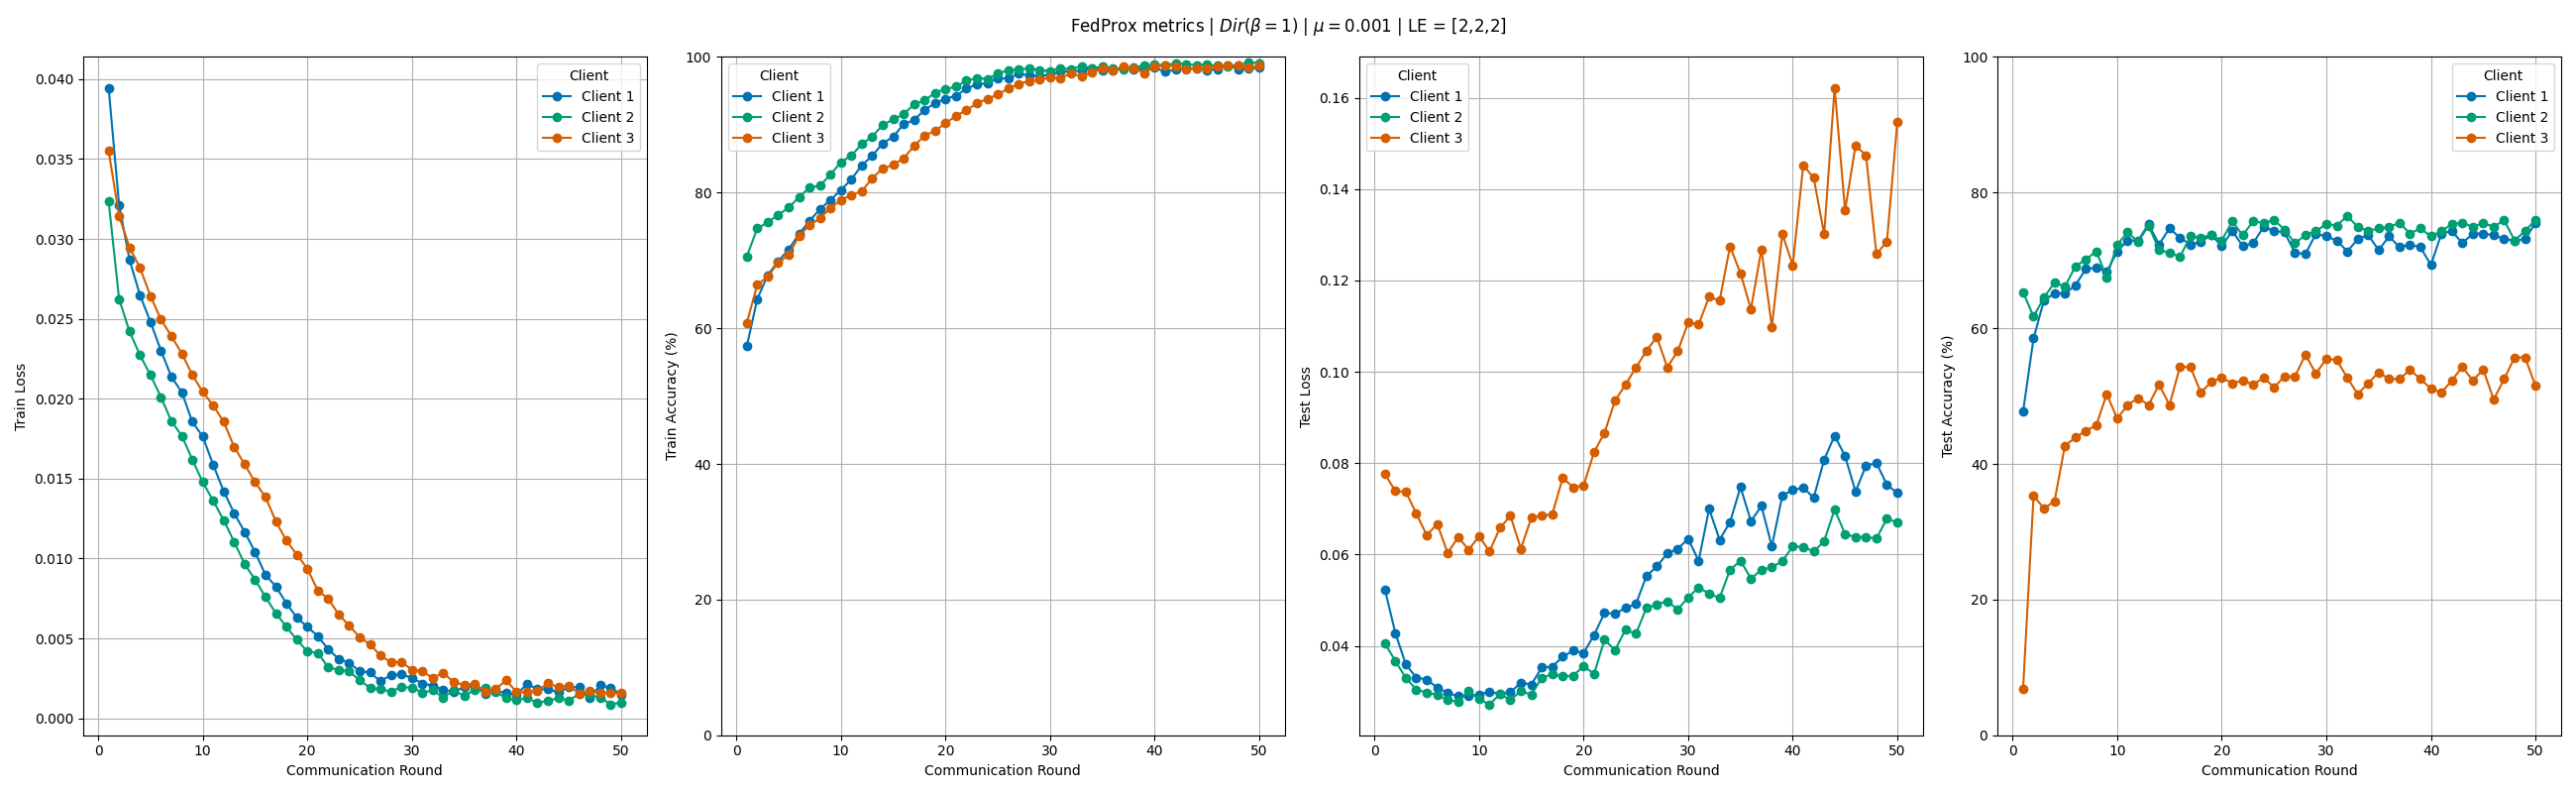
\includegraphics[width=0.8\linewidth]{figures/2-Federated_Learning/FedProx_Dirichlet_1_mu_0.001.png}
    \end{subfigure}
    \vspace{1em} % Space between images

    \begin{subfigure}{\linewidth}
        \centering
        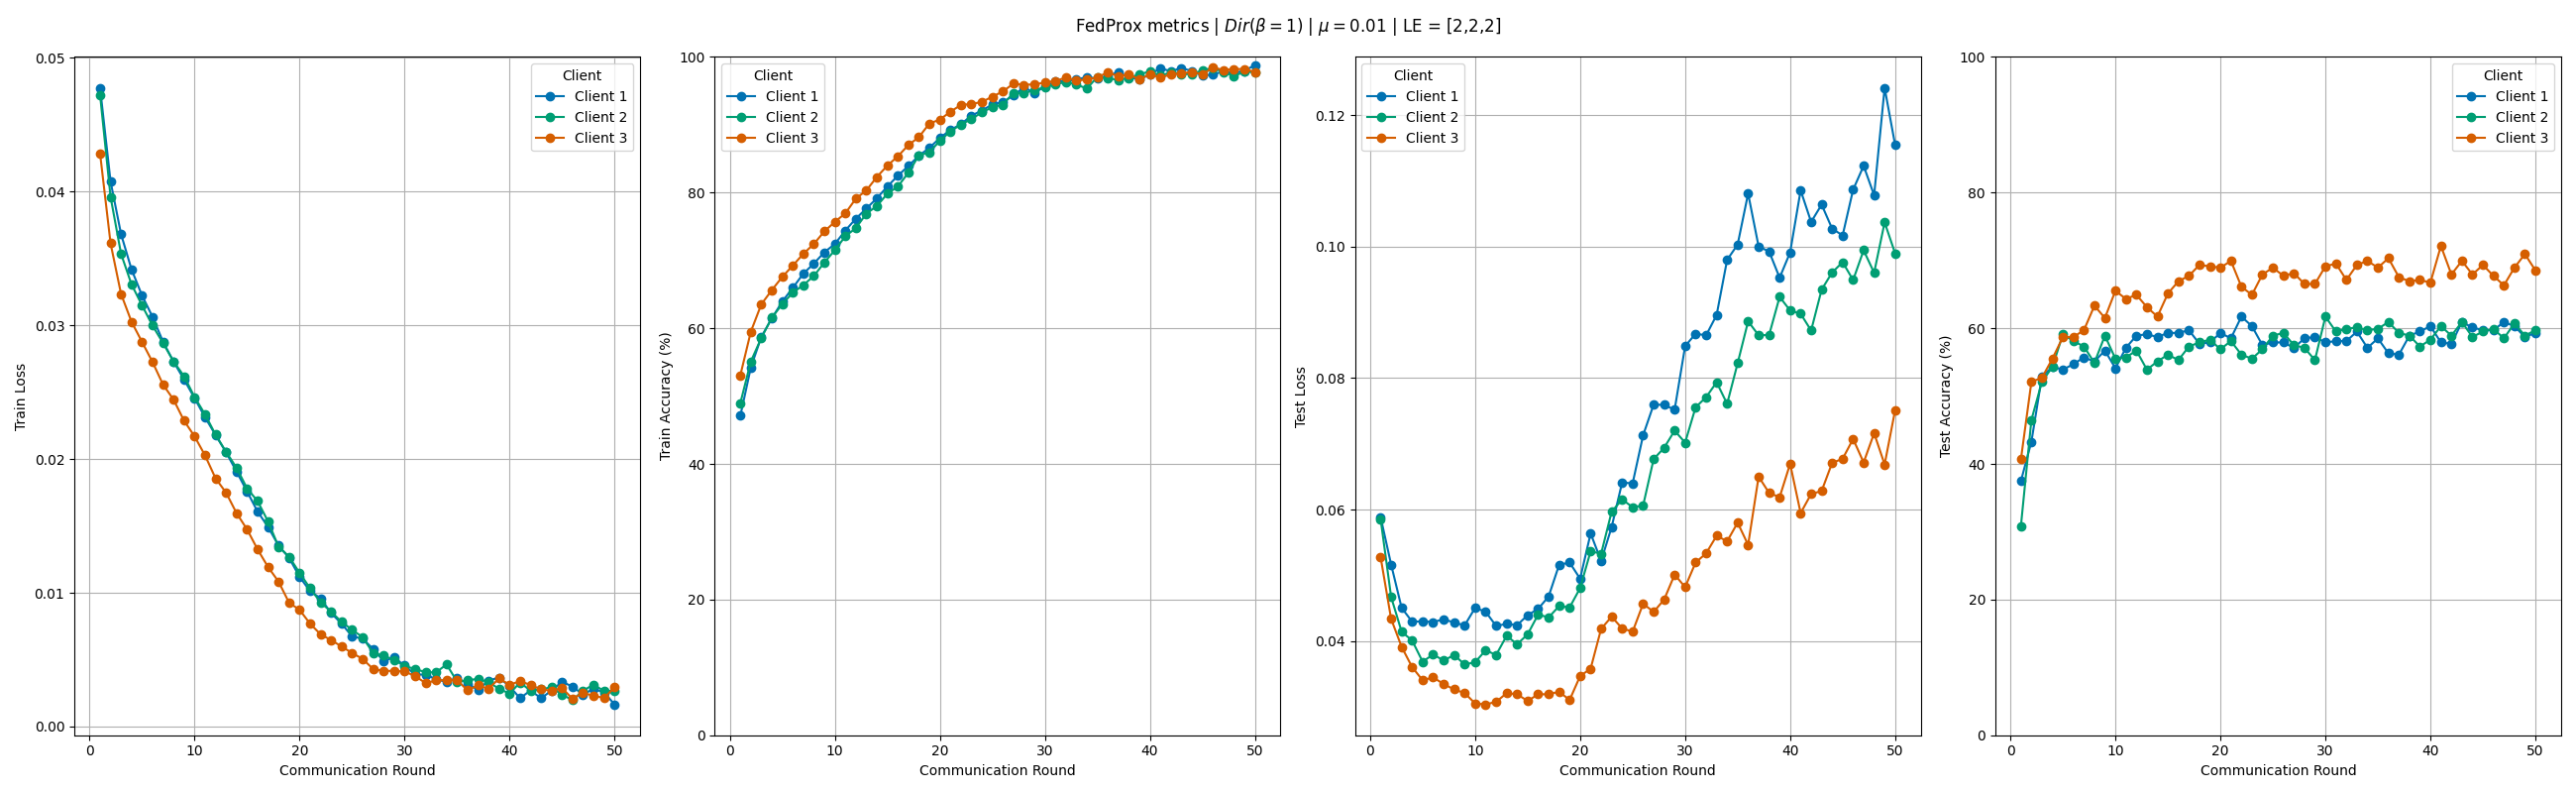
\includegraphics[width=0.8\linewidth]{figures/2-Federated_Learning/FedProx_Dirichlet_1_mu_0.01.png}
    \end{subfigure}
    \vspace{1em} % Space between images

    \begin{subfigure}{\linewidth}
        \centering
        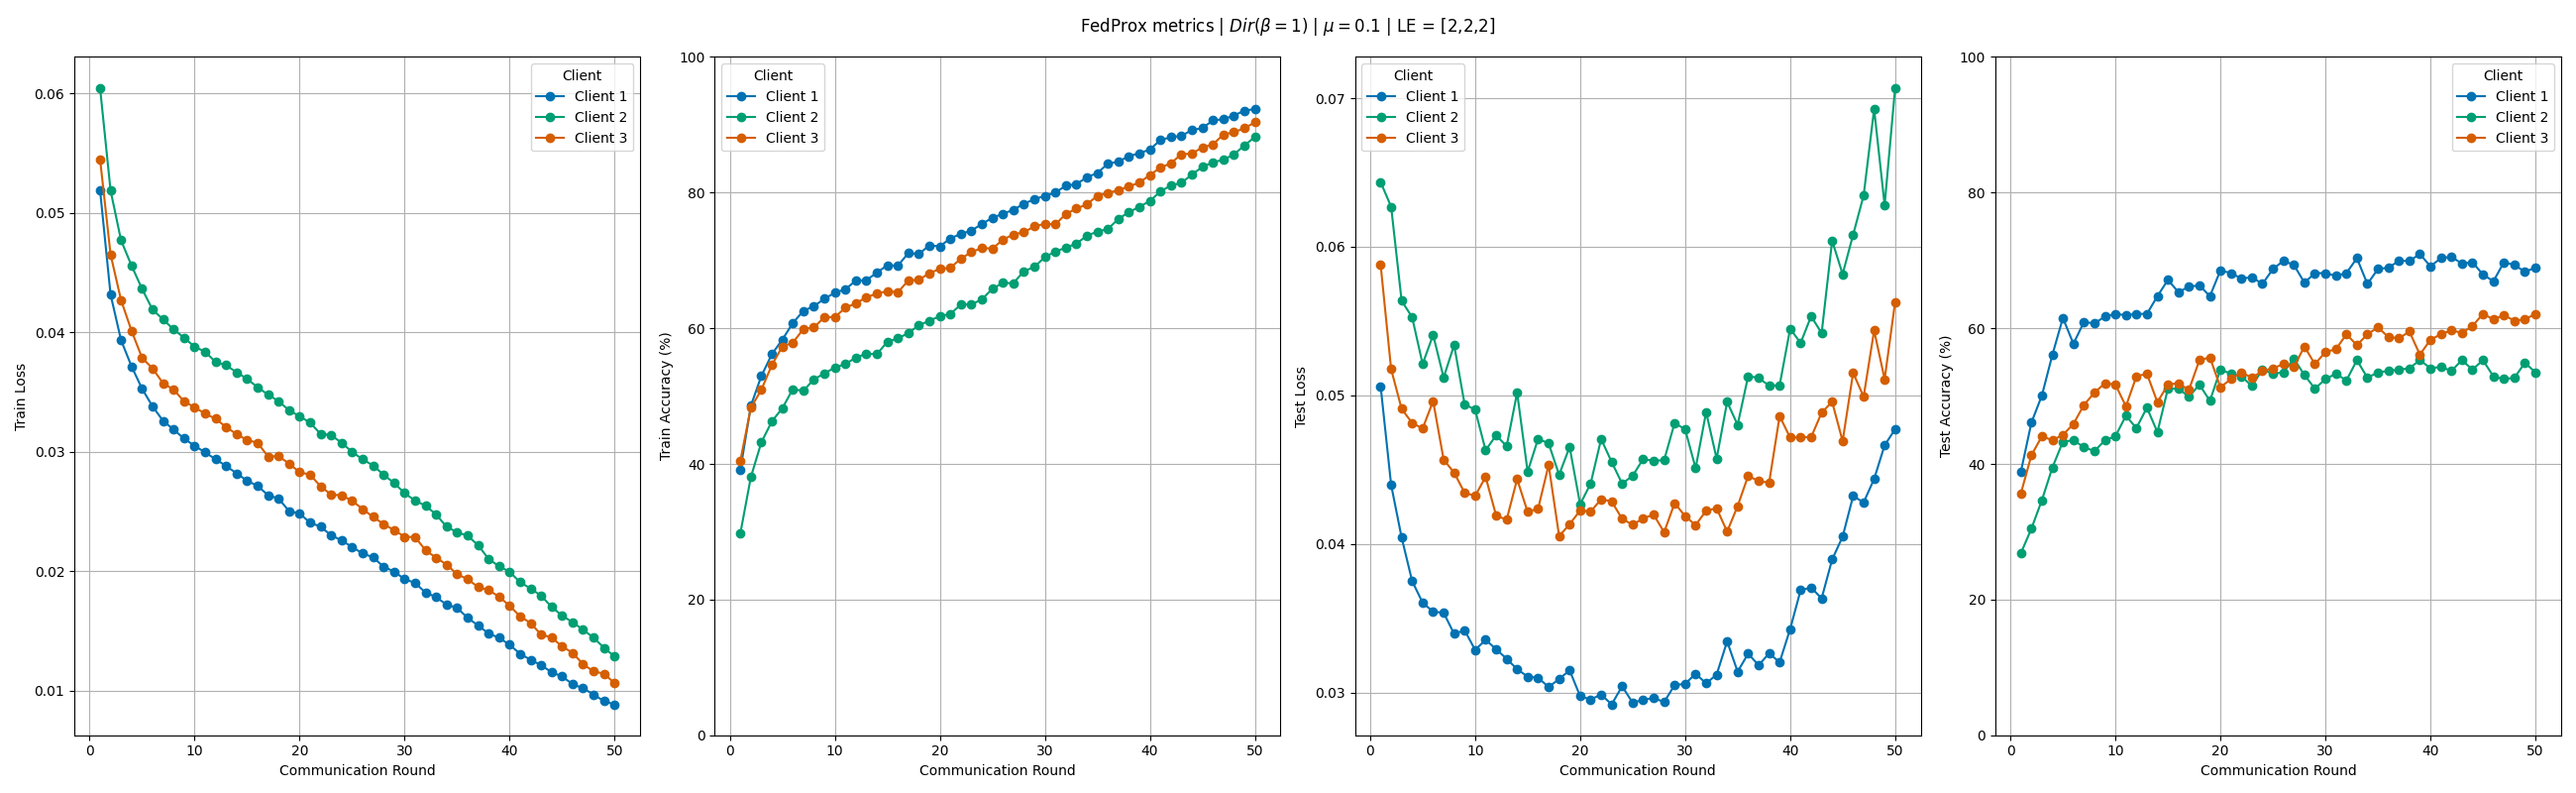
\includegraphics[width=0.8\linewidth]{figures/2-Federated_Learning/FedProx_Dirichlet_1_mu_0.1.png}
    \end{subfigure}
    \vspace{1em} % Space between images

    \begin{subfigure}{\linewidth}
        \centering
        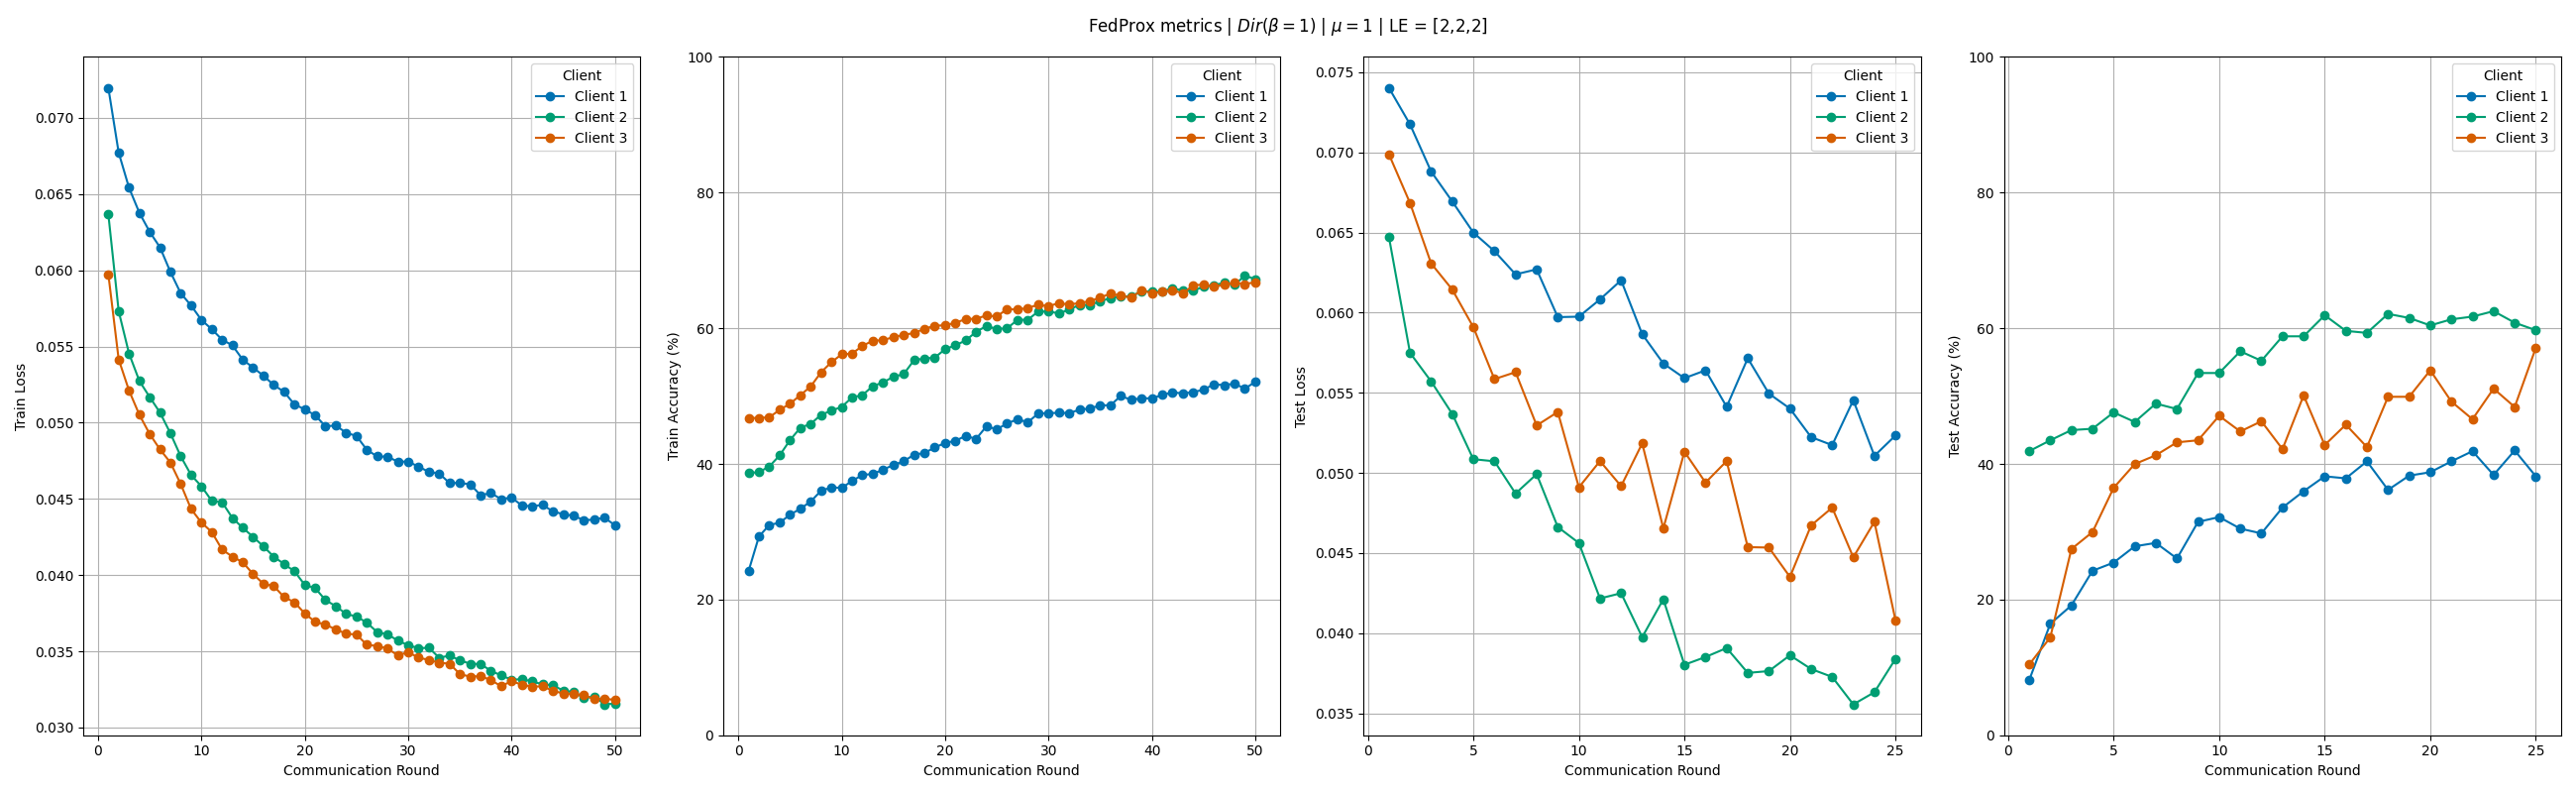
\includegraphics[width=0.8\linewidth]{figures/2-Federated_Learning/FedProx_Dirichlet_1_mu_1.png}
    \end{subfigure}

    \caption{Local metrics for 3 clients in 50 communication rounds using FedProx with a Non-IID setting over the CIFAR10 dataset, $\mu \in \{0.001, 0.01, 0.1, 1\}$. Label distribution skew using the Dirichlet distribution with $\boldsymbol{\beta} = (1,1,1)$ }
    \label{fig:FedProx_Non_IID_Dirichlet_1}
\end{figure}


\begin{figure}[H]
    \centering

    \begin{subfigure}{\linewidth}
        \centering
        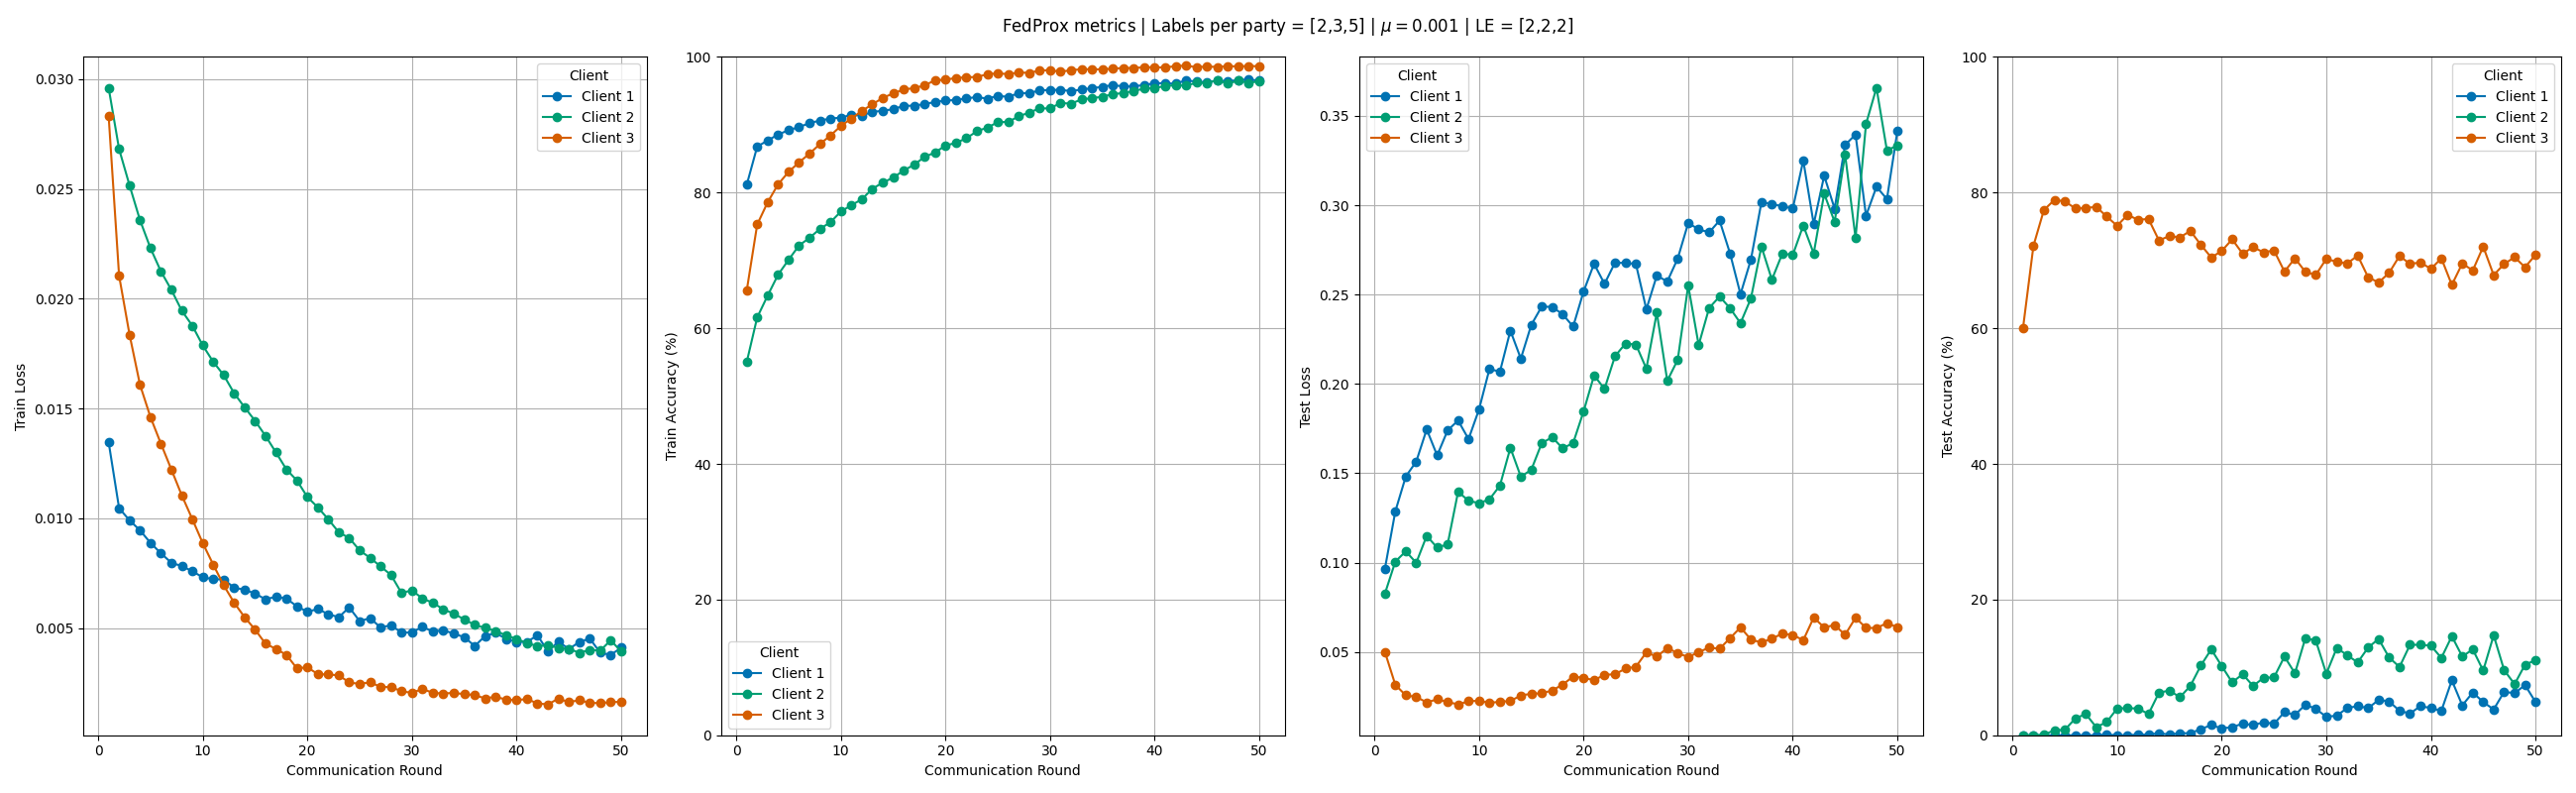
\includegraphics[width=0.8\linewidth]{figures/2-Federated_Learning/FedProx_LabelsPerParty_mu_0.001.png}
    \end{subfigure}
    \vspace{1em} % Space between images

    \begin{subfigure}{\linewidth}
        \centering
        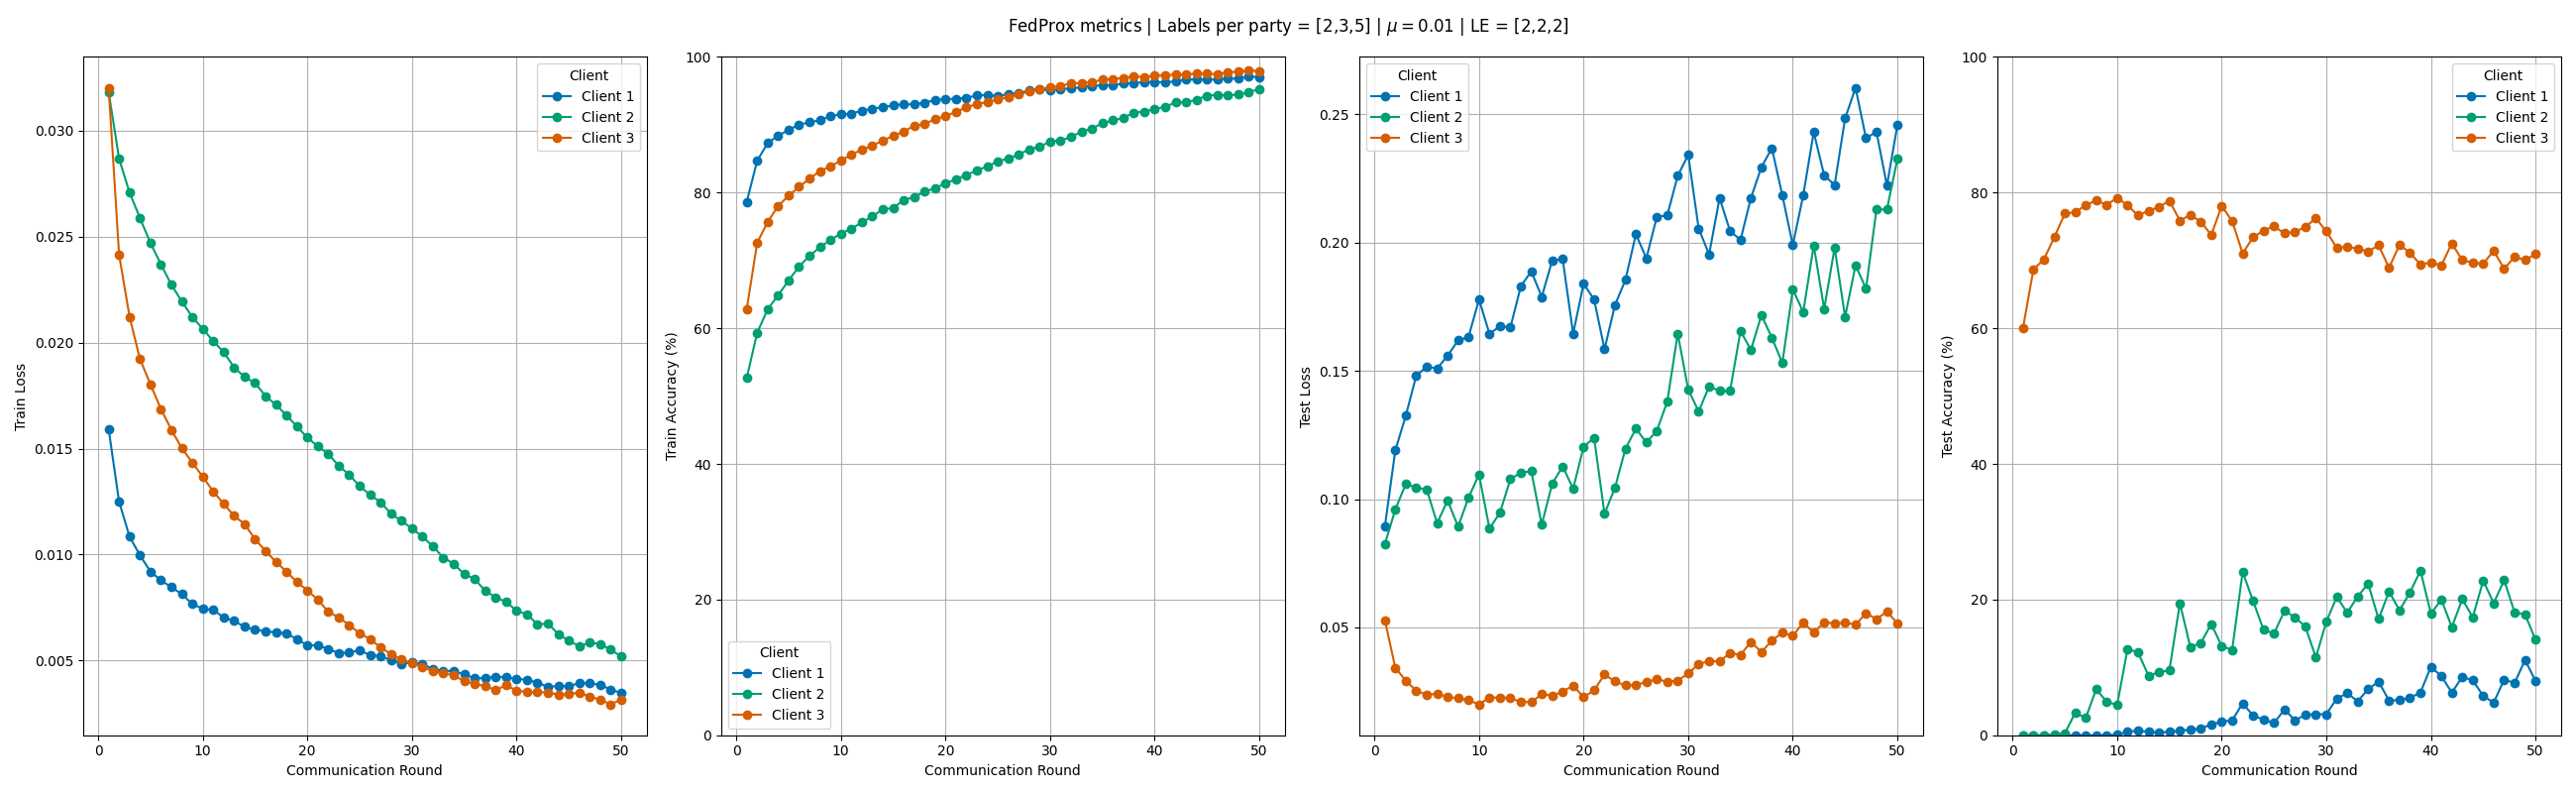
\includegraphics[width=0.8\linewidth]{figures/2-Federated_Learning/FedProx_LabelsPerParty_mu_0.01.png}
    \end{subfigure}
    \vspace{1em} % Space between images

    \begin{subfigure}{\linewidth}
        \centering
        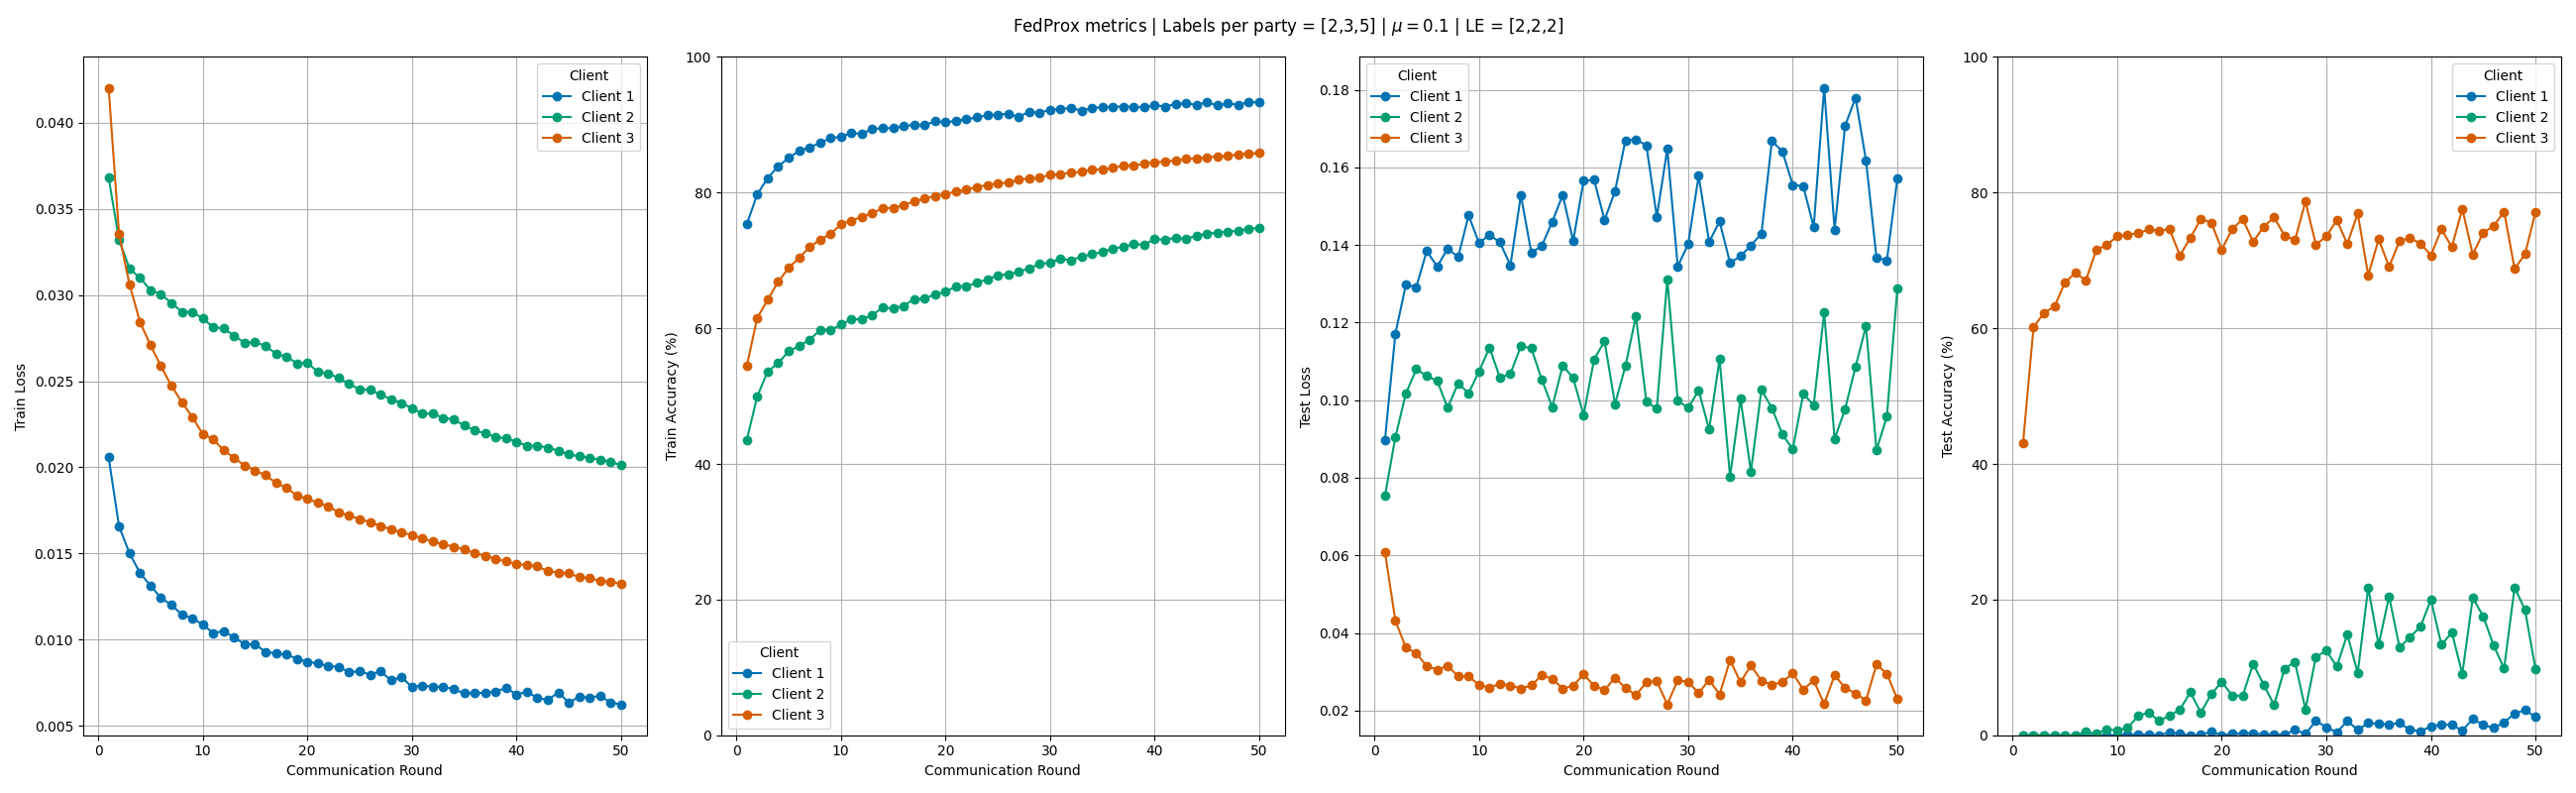
\includegraphics[width=0.8\linewidth]{figures/2-Federated_Learning/FedProx_LabelsPerParty_mu_0.1.png}
    \end{subfigure}
    \vspace{1em} % Space between images

    \begin{subfigure}{\linewidth}
        \centering
        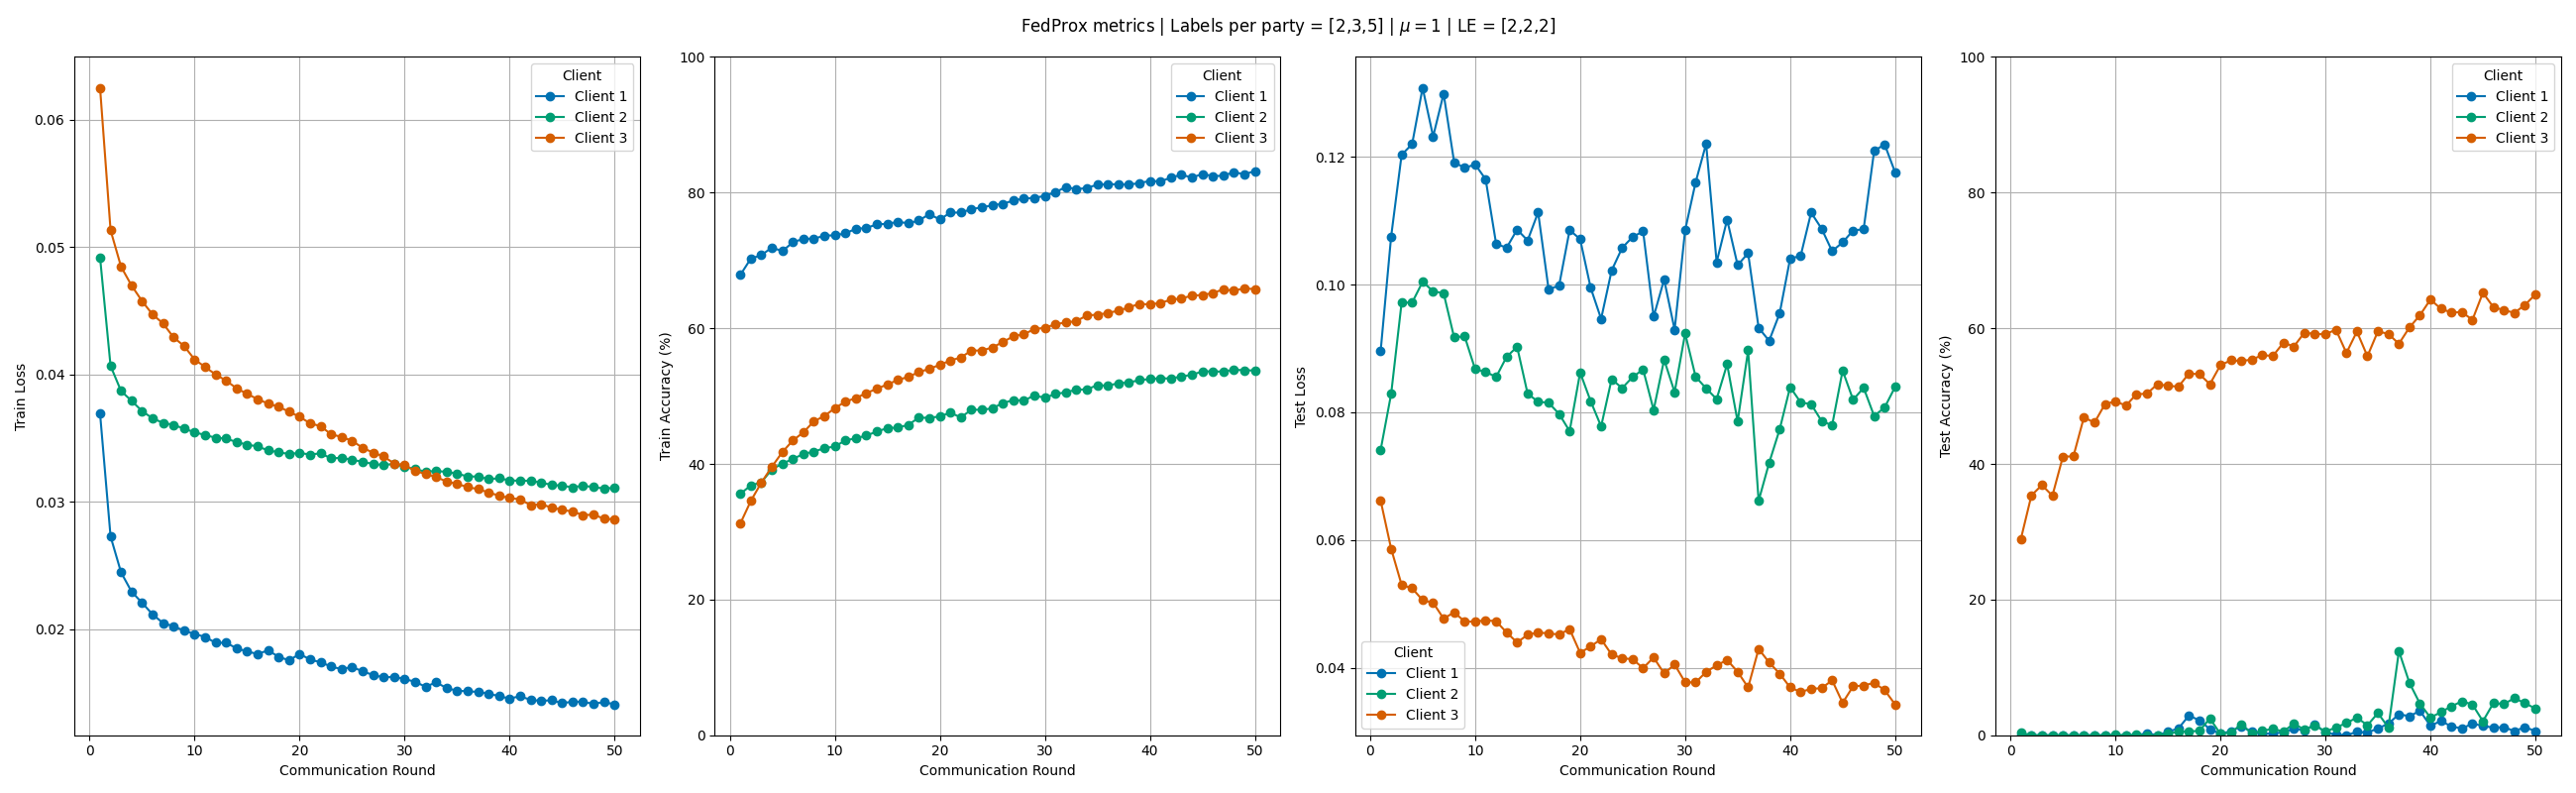
\includegraphics[width=0.8\linewidth]{figures/2-Federated_Learning/FedProx_LabelsPerParty_mu_1.png}
    \end{subfigure}

    \caption{Local metrics for 3 clients in 50 communication rounds using FedProx with a Non-IID setting over the CIFAR10 dataset, $\mu \in \{0.001, 0.01, 0.1, 1\}$.  Label distribution skew, the first client data from 2 classes, the second client
from 3 classes and the third client from the 5 remaining classes.}
    \label{fig:FedProx_Non_IID_LabelsPerParty}
\end{figure}




\begin{figure}[H]
    \centering

    \begin{subfigure}{\linewidth}
        \centering
        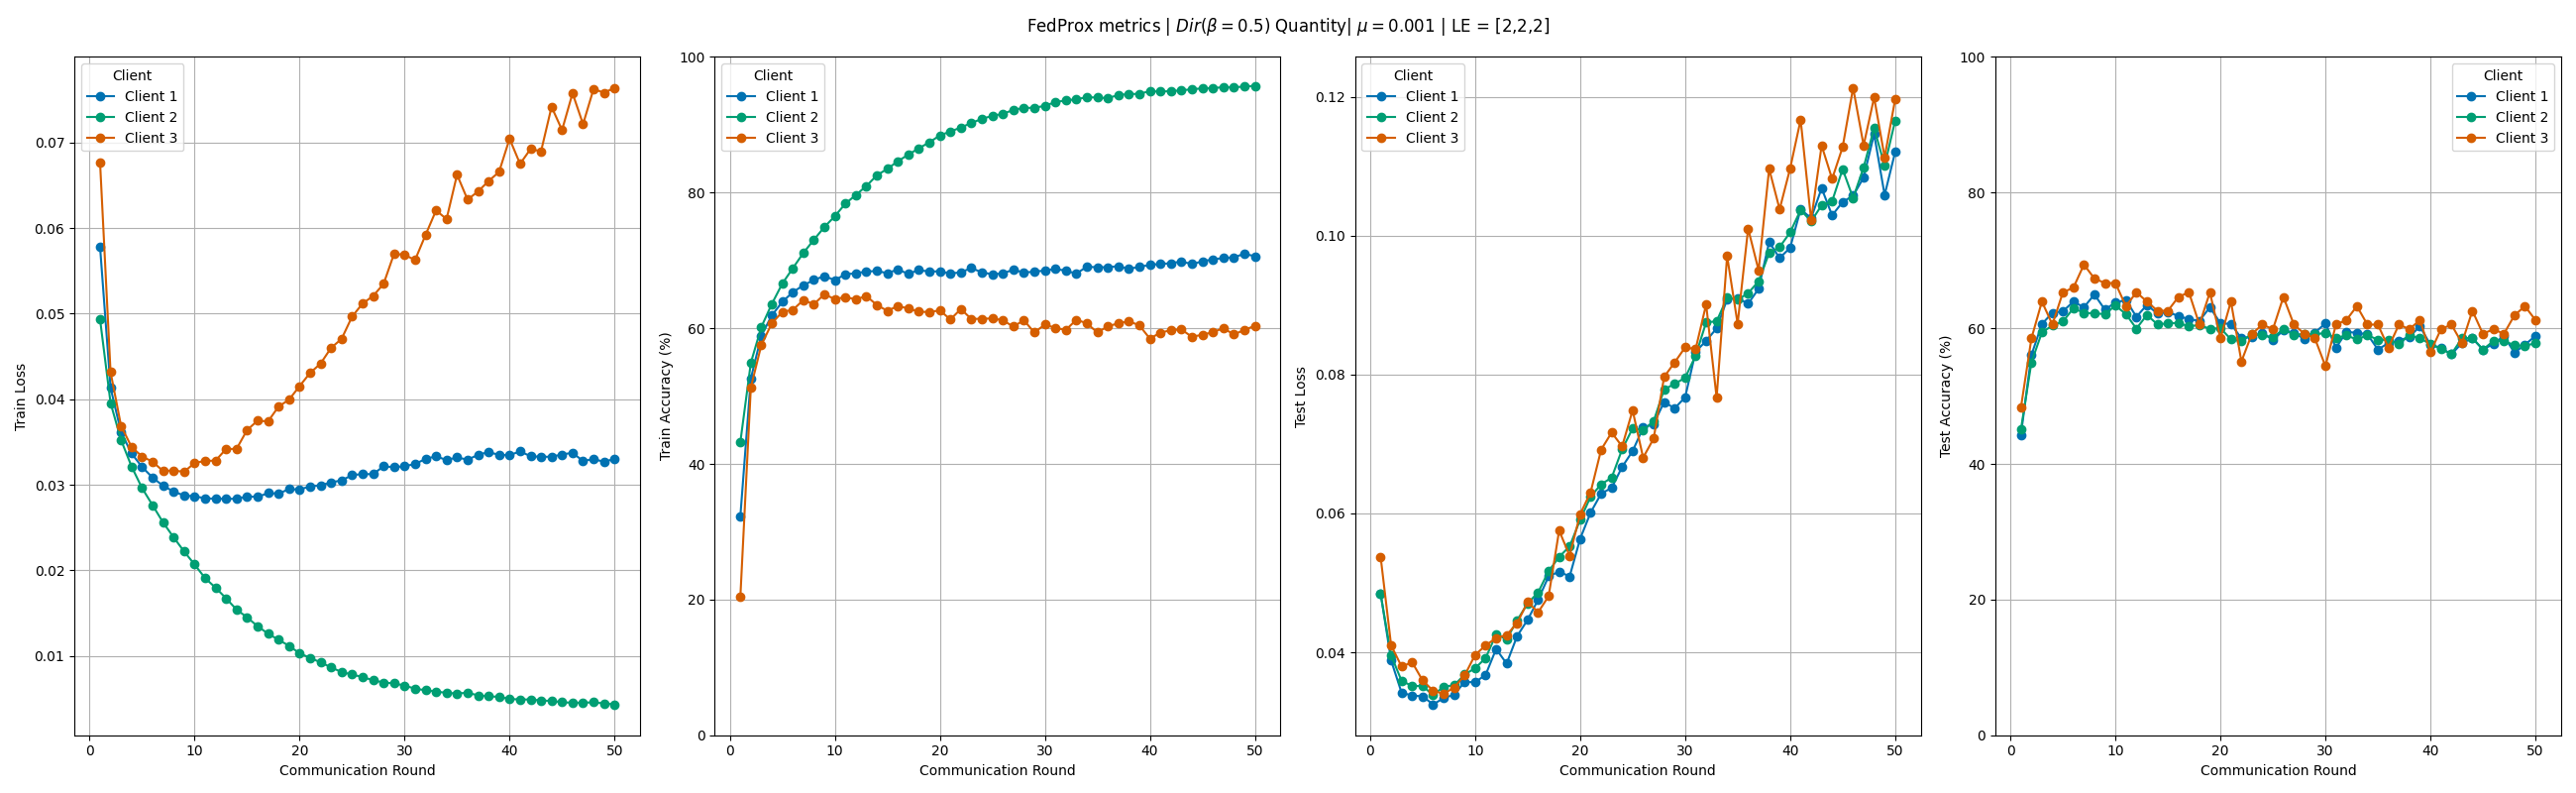
\includegraphics[width=0.8\linewidth]{figures/2-Federated_Learning/FedProx_QuantitySkew_Dir_05_Mu_0.001.png}
    \end{subfigure}
    \vspace{1em} % Space between images

    \begin{subfigure}{\linewidth}
        \centering
        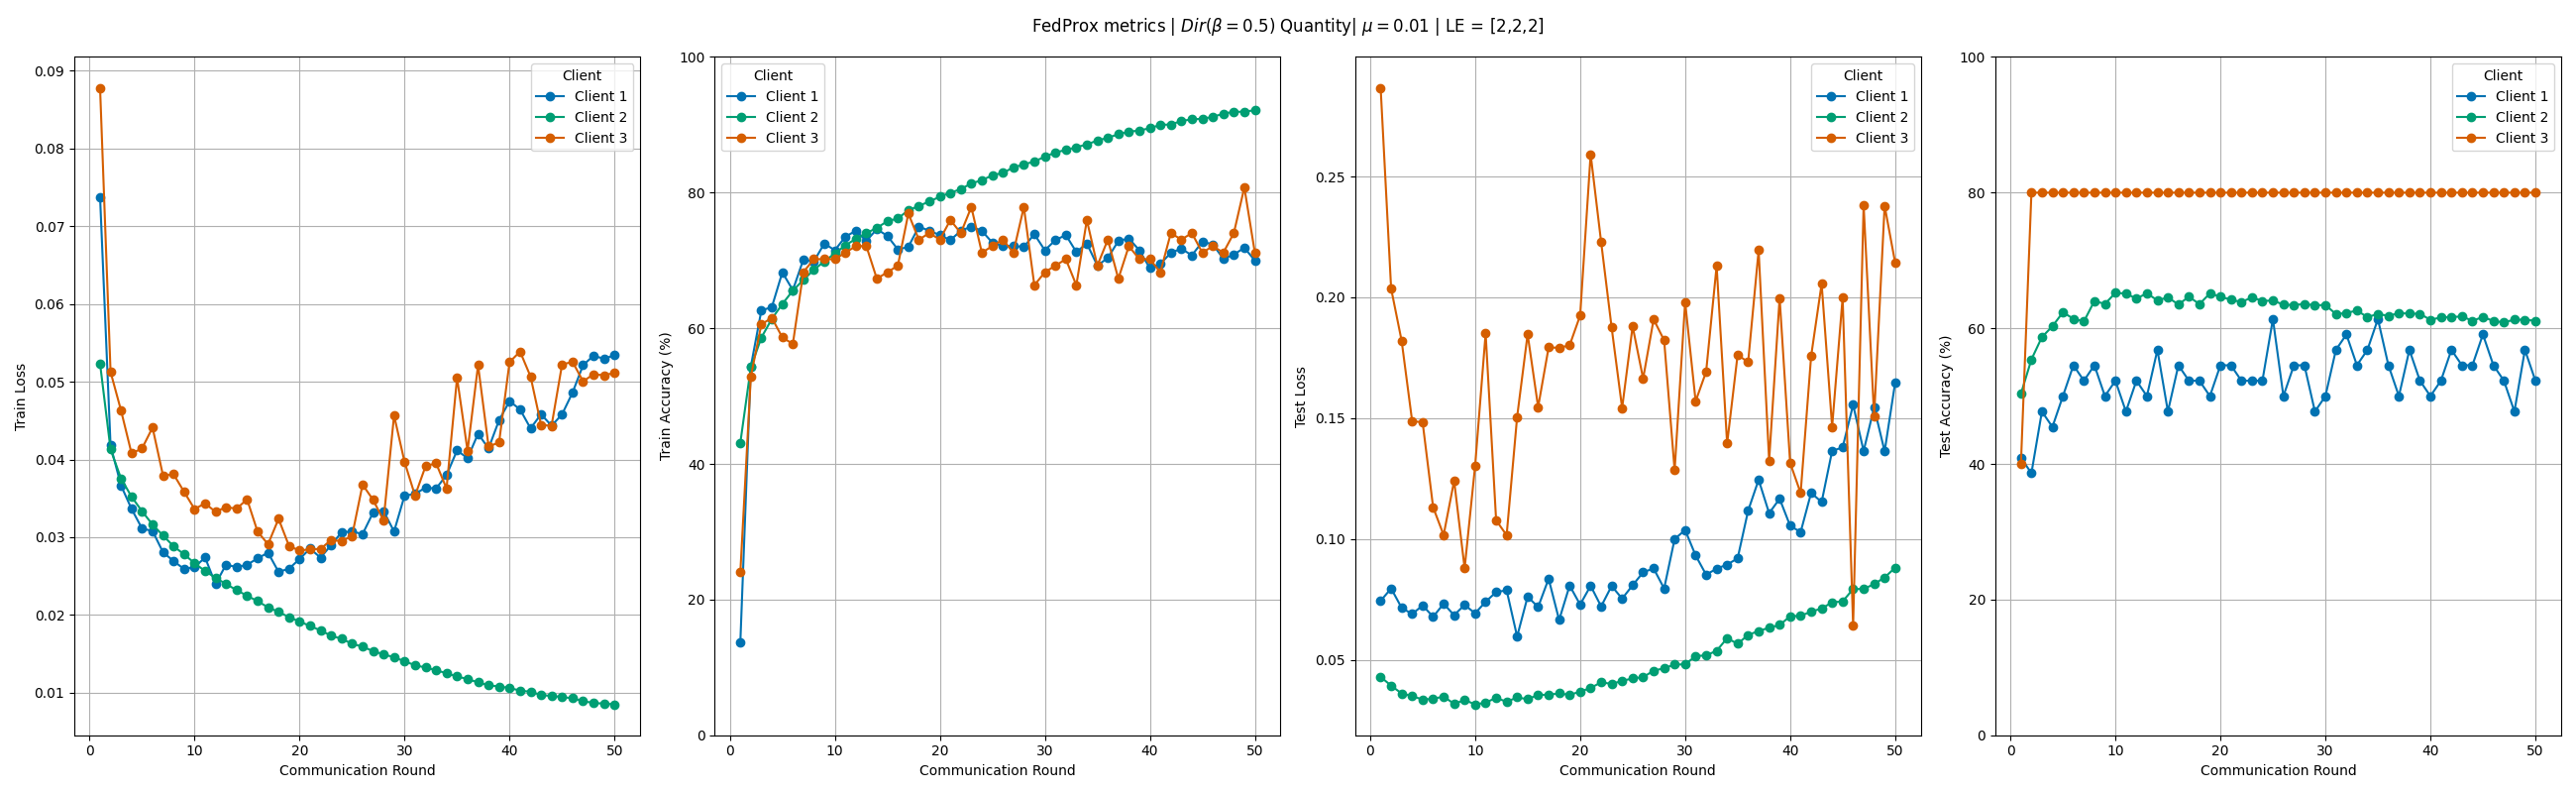
\includegraphics[width=0.8\linewidth]{figures/2-Federated_Learning/FedProx_QuantitySkew_Dir_05_Mu_0.01.png}
    \end{subfigure}
    \vspace{1em} % Space between images

    \begin{subfigure}{\linewidth}
        \centering
        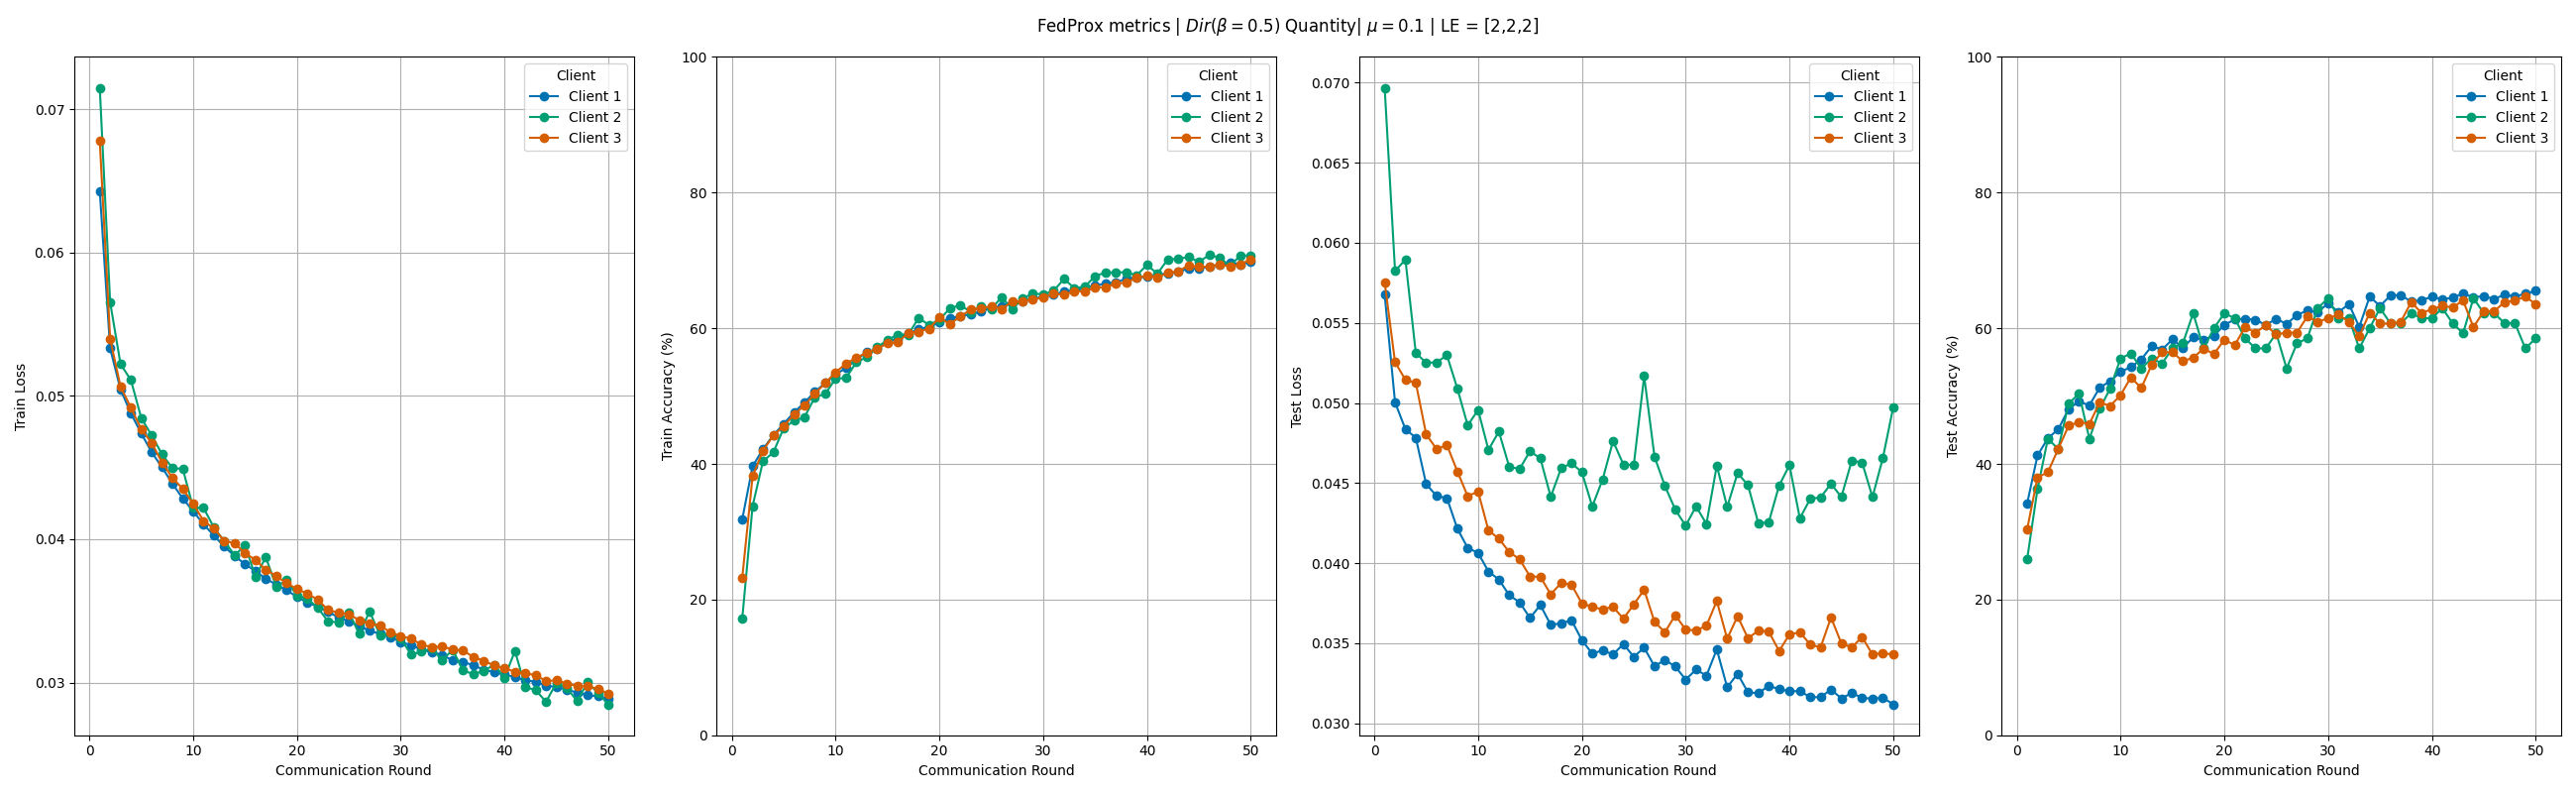
\includegraphics[width=0.8\linewidth]{figures/2-Federated_Learning/FedProx_QuantitySkew_Dir_05_Mu_0.1.png}
    \end{subfigure}
    \vspace{1em} % Space between images

    \begin{subfigure}{\linewidth}
        \centering
        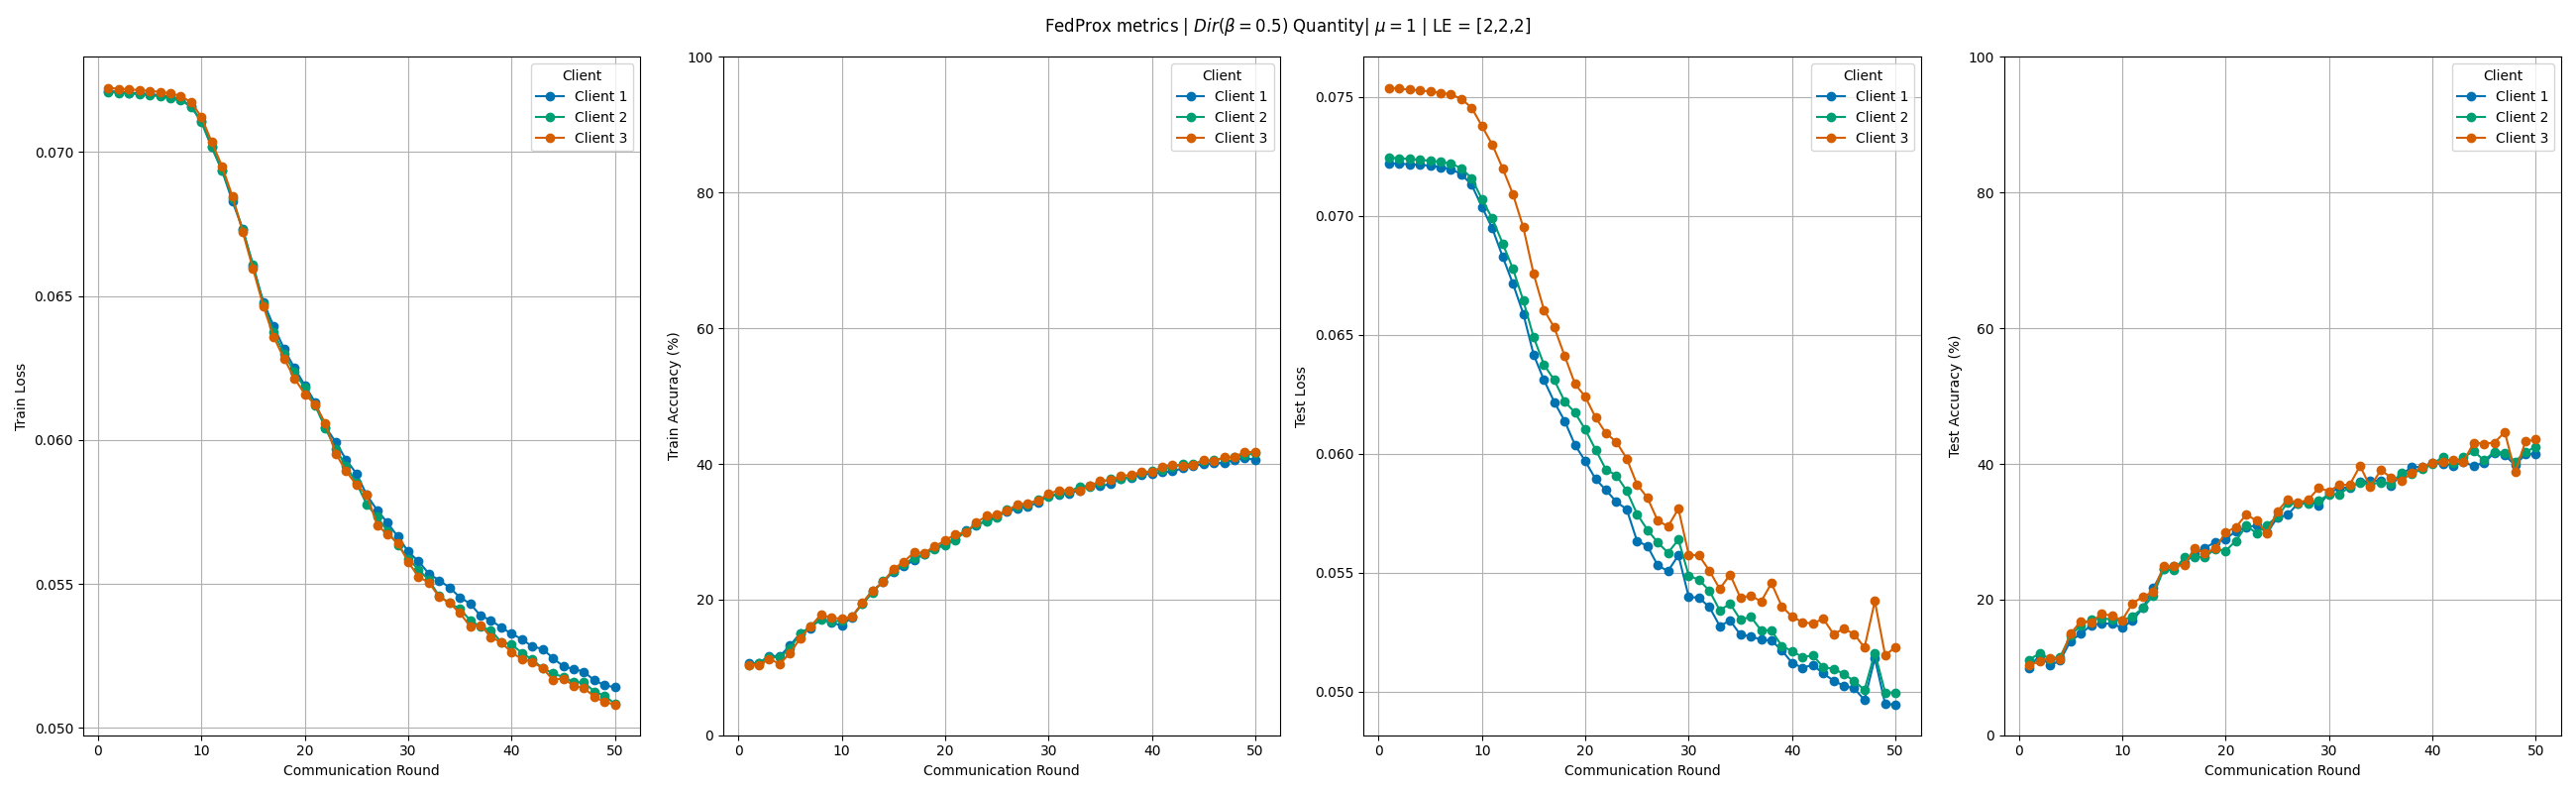
\includegraphics[width=0.8\linewidth]{figures/2-Federated_Learning/FedProx_QuantitySkew_Dir_05_Mu_1.png}
    \end{subfigure}

    \caption{Local metrics for 3 clients in 50 communication rounds using FedProx with a Non-IID setting over the CIFAR10 dataset, $\mu \in \{0.001, 0.01, 0.1, 1\}$.  Label quantity distribution skew using $Dir(\boldsymbol{\beta})$, $\boldsymbol{\beta} = (0.5,0.5,0.5)$  }
    \label{fig:FedProx_Non_IID_LabelQuantitySkeqDir_05}
\end{figure}




\begin{figure}[H]
    \centering

    \begin{subfigure}{\linewidth}
        \centering
        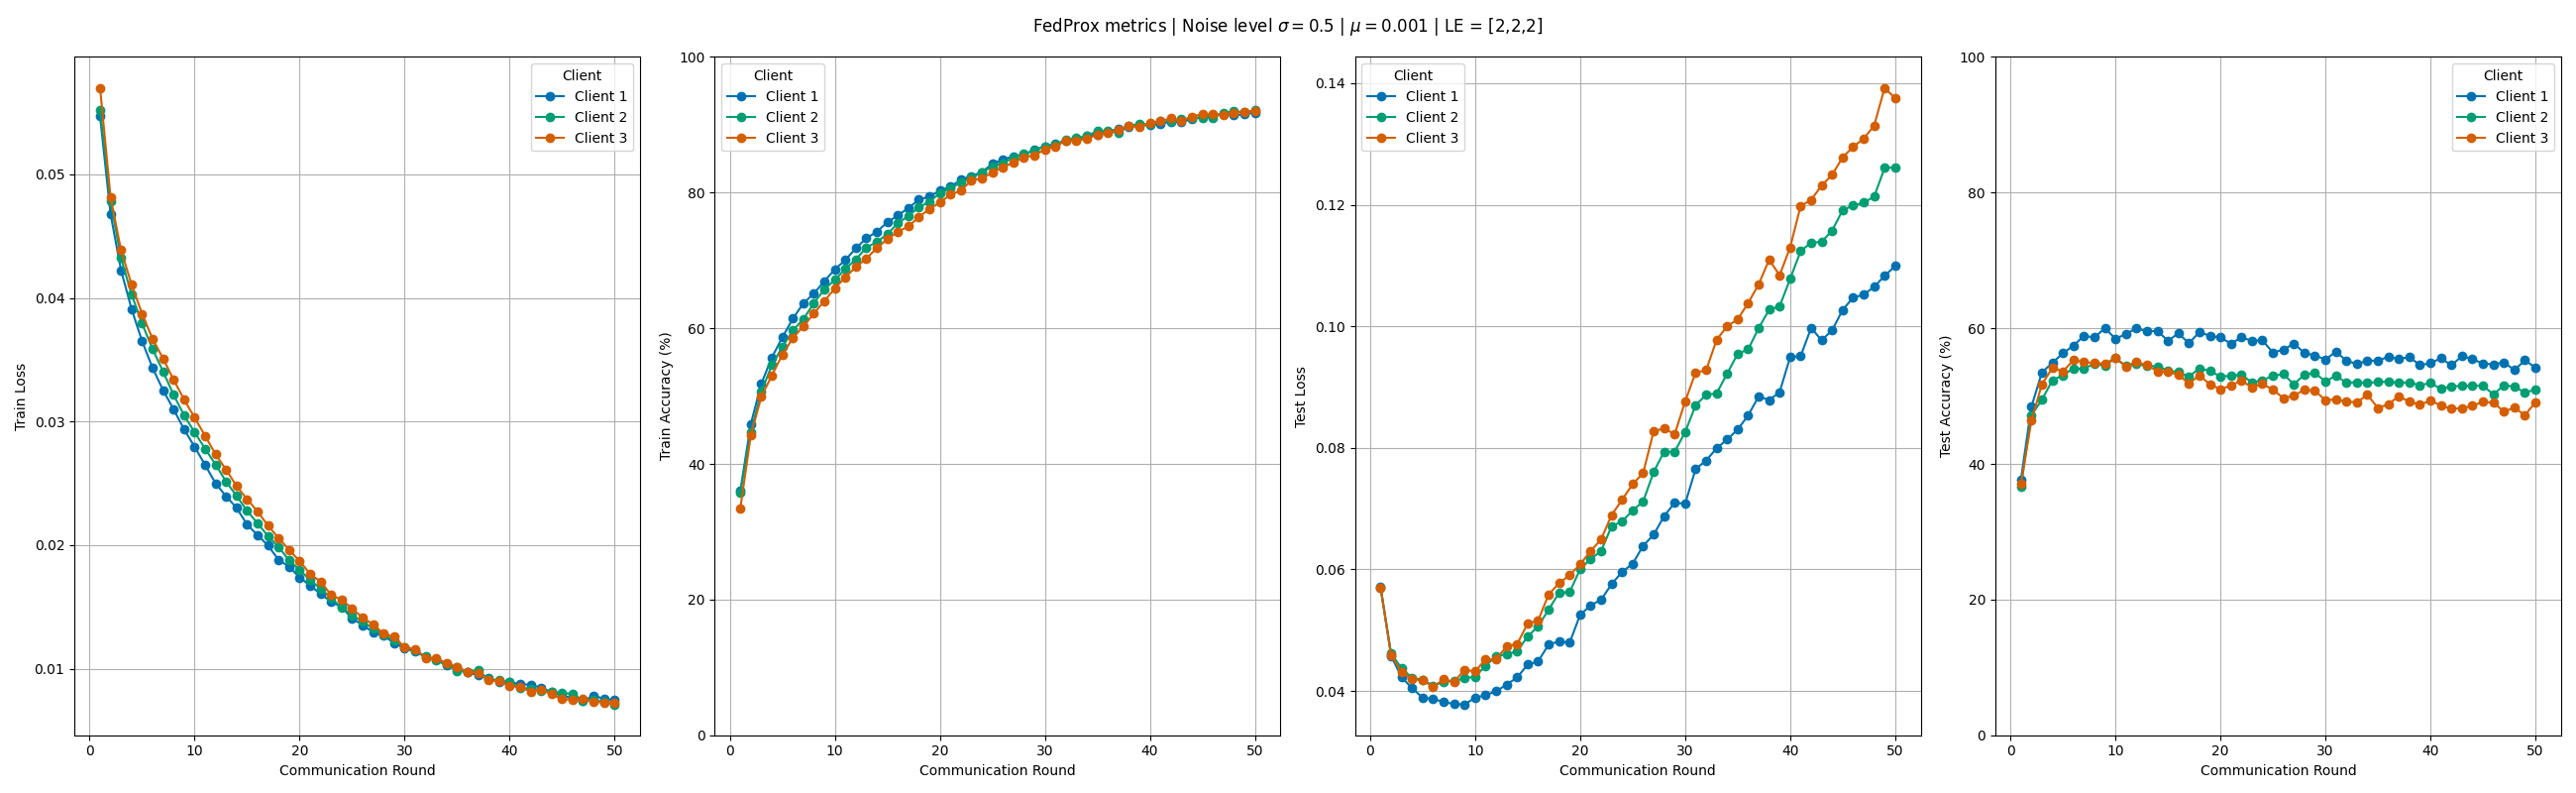
\includegraphics[width=0.8\linewidth]{figures/2-Federated_Learning/FedProx_NoiseLevel_Mu_0.001.png}
    \end{subfigure}
    \vspace{1em} % Space between images

    \begin{subfigure}{\linewidth}
        \centering
        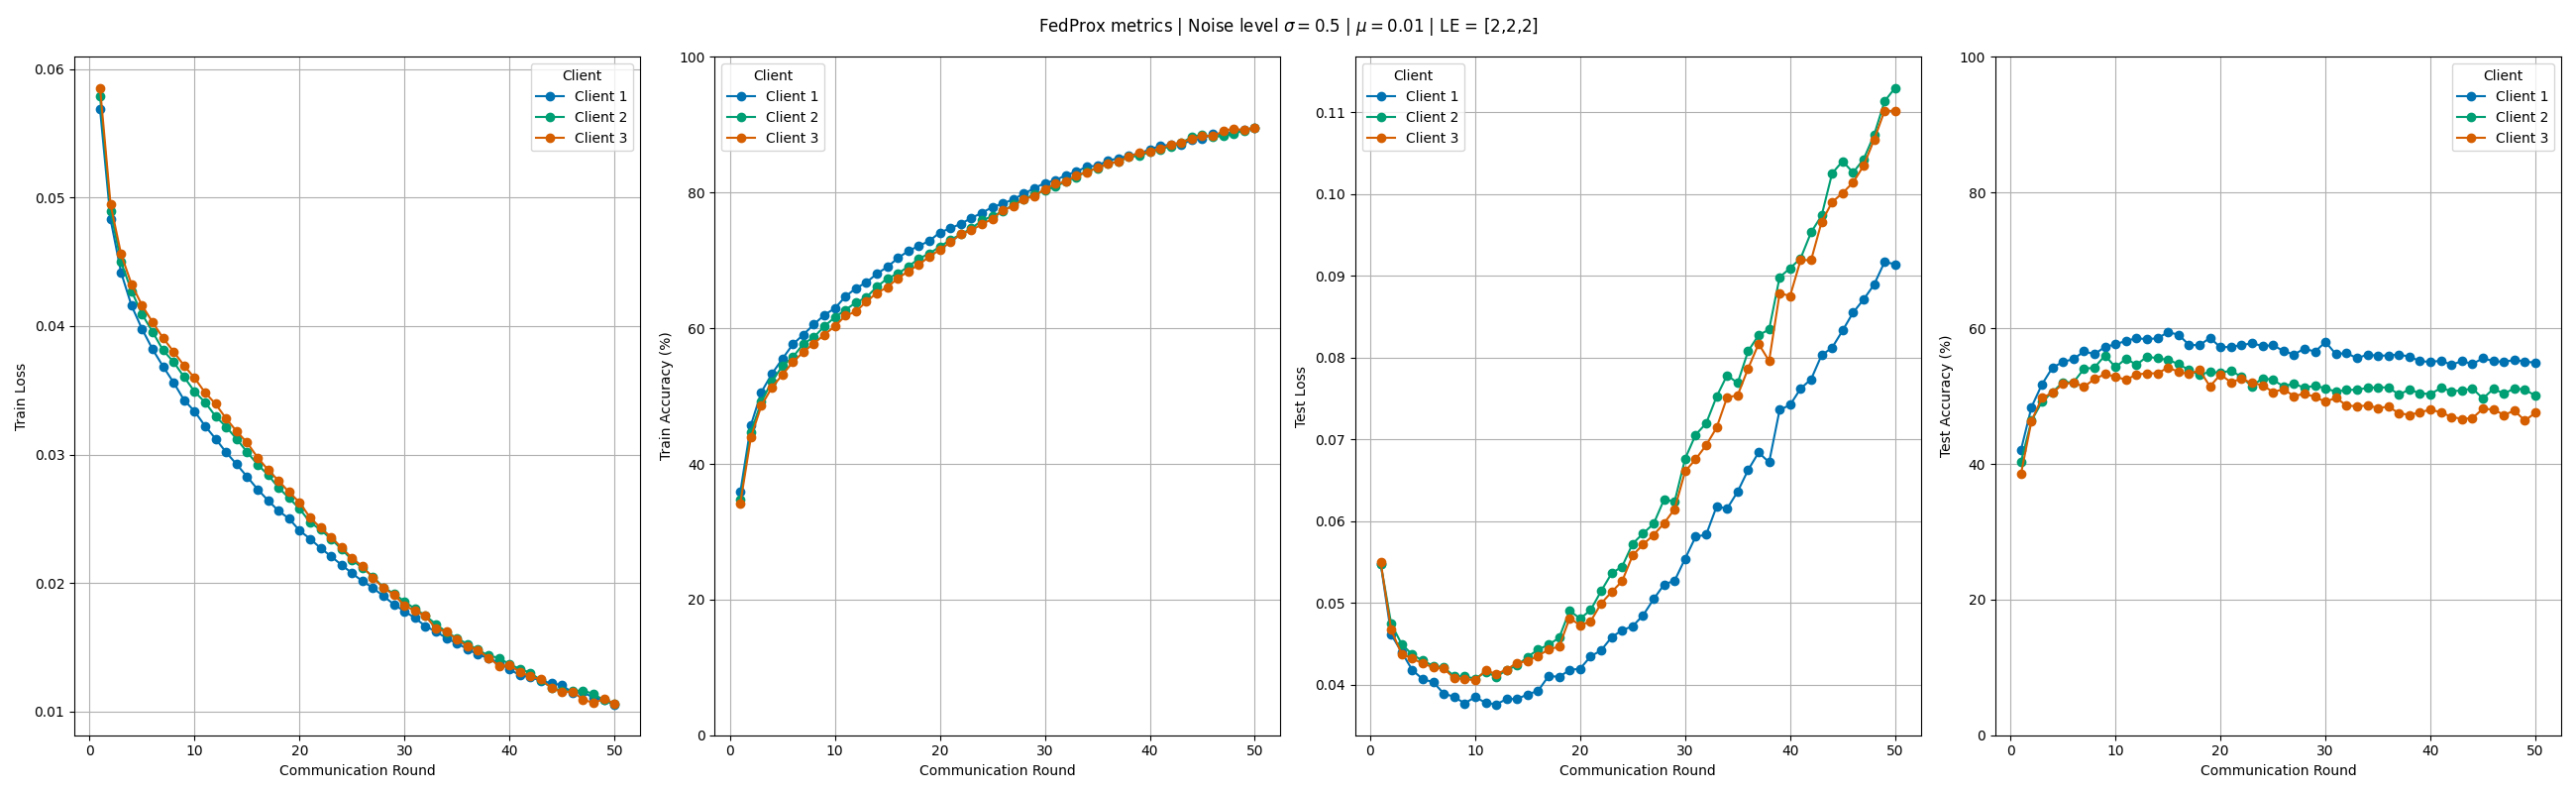
\includegraphics[width=0.8\linewidth]{figures/2-Federated_Learning/FedProx_NoiseLevel_Mu_0.01.png}
    \end{subfigure}
    \vspace{1em} % Space between images

    \begin{subfigure}{\linewidth}
        \centering
        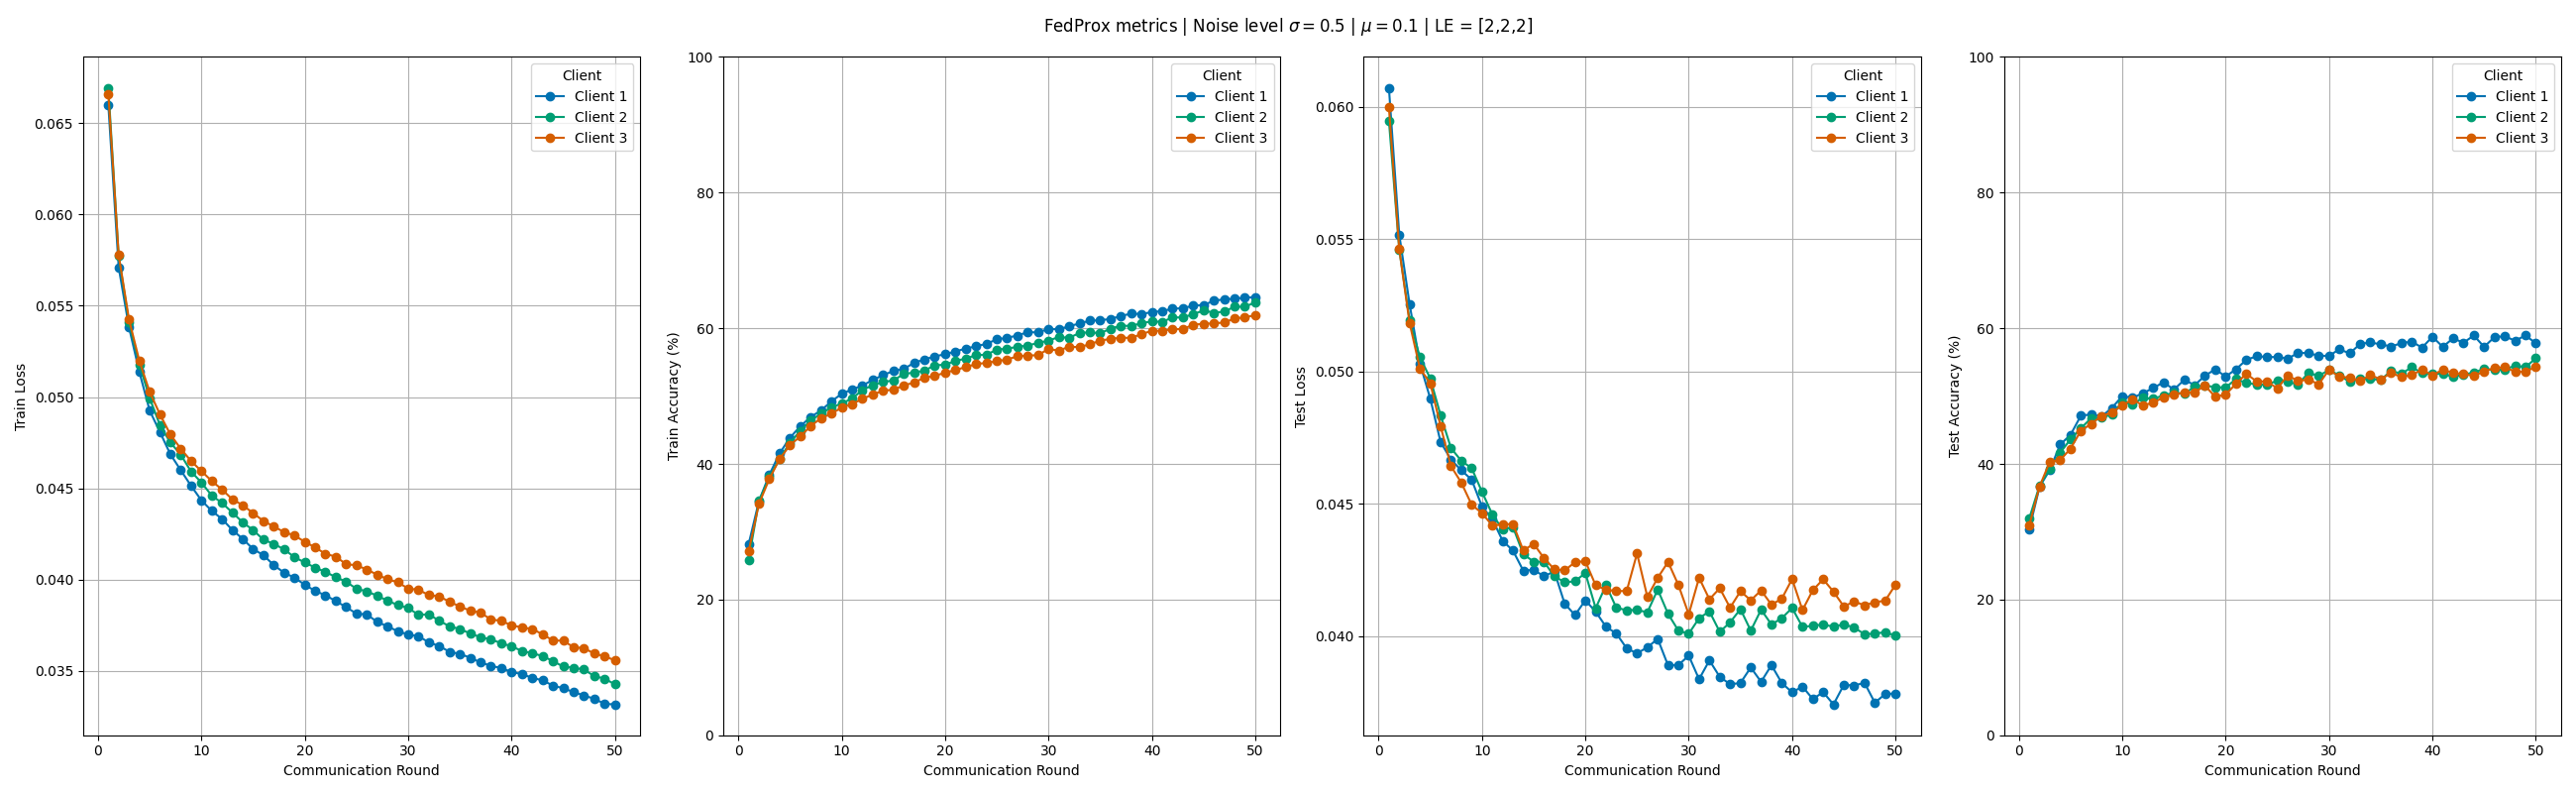
\includegraphics[width=0.8\linewidth]{figures/2-Federated_Learning/FedProx_NoiseLevel_Mu_0.1.png}
    \end{subfigure}
    \vspace{1em} % Space between images

    \begin{subfigure}{\linewidth}
        \centering
        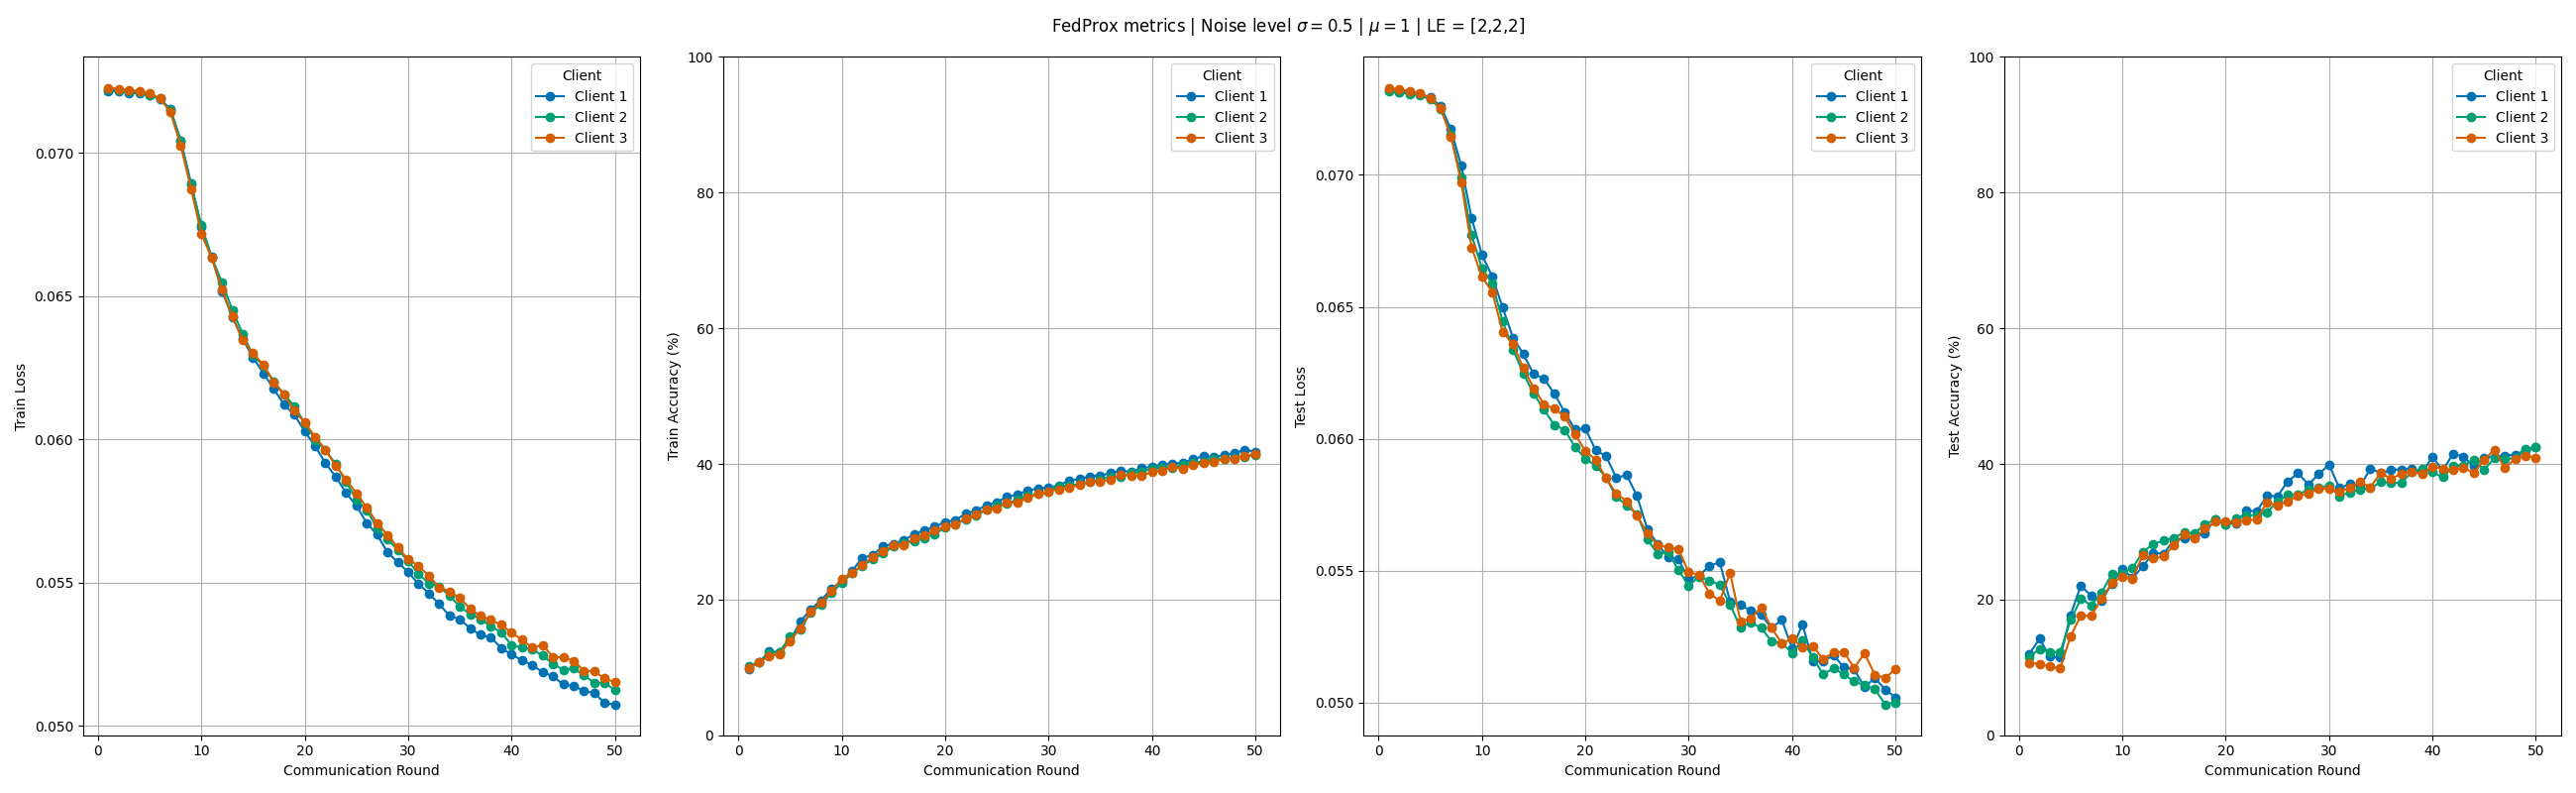
\includegraphics[width=0.8\linewidth]{figures/2-Federated_Learning/FedProx_NoiseLevel_Mu_1.png}
    \end{subfigure}

    \caption{Local metrics for 3 clients in 50 communication rounds using FedProx with a Non-IID setting over the CIFAR10 dataset, $\mu \in \{0.001, 0.01, 0.1, 1\}$. Feature distribution skew using with noise level $\sigma = 0.5$}
    \label{fig:FedProx_Non_IID_NoiseLevel_05}
\end{figure}


\printbibliography
\end{document}
